% !TeX program = pdflatex
\documentclass{iutbscthesis}
\usepackage{comment}
\usepackage{multirow}
\usepackage{tabularx}
\usepackage{float}

\addbibresource{citations.bib}

% Project Title
\title{Deep Reinforcement Learning for Autonomous Vehicle Navigation at Unsignalized Intersections: Comparative Reproduction, Intent Encoding, and Sim-to-Sim Dynamics}

% Authors (Configurable with student names and IDs)
\addauthor{Farhan Tahsin Khan}{220041229}
\addauthor{Mahmudul Hasan}{220041231}
\addauthor{A.K.M Ishmam Tahmid}{220041259}

% Supervision
\supervisor{Supervisor Name}{Professor / Associate Professor}{Department of Computer Science and Engineering}
%\addcosupervisor{Co-Supervisor Name}{Assistant Professor}{Department of Computer Science and Engineering}

% Academic Program and Department
\department{Department of Computer Science and Engineering}
\program{BACHELOR OF SCIENCE IN COMPUTER SCIENCE AND ENGINEERING}
\defensedate{15}{October}{2026}

\begin{document}

%-------------------------- FRONT MATTER --------------------------%
\pagenumbering{roman}

% Title leaf
\titlepage

\setcounter{tocdepth}{1}
\begingroup
\begin{singlespace}
\linespread{0.88}\selectfont
\makeatletter
\renewcommand*\l@chapter[2]{%
  \ifnum \c@tocdepth >\m@ne
    \vskip 0.12em \@plus\p@
    \setlength\@tempdima{1.5em}%
    \begingroup
      \parindent \z@ \rightskip \@pnumwidth
      \parfillskip -\@pnumwidth
      \leavevmode \bfseries
      \advance\leftskip\@tempdima
      \hskip -\leftskip
      #1\nobreak\hfil \nobreak\hb@xt@\@pnumwidth{\hss #2}\par
    \endgroup
  \fi}
\makeatother
\footnotesize
\tableofcontents
\end{singlespace}
\endgroup
\clearpage

% Combined List of Figures and Tables
\begingroup
\begin{singlespace}
\small
\let\clearpage\relax
\let\cleardoublepage\relax
\vspace*{-0.5cm}
\listoffigures
\vspace{0.4cm}
\listoftables
\end{singlespace}
\endgroup
\clearpage

% Abbreviations
\begin{abbreviations}
    \abbr{AEV}{Autonomous Electric Vehicle}
    \abbr{AIM}{Autonomous Intersection Management}
    \abbr{CAV}{Connected and Automated Vehicle}
    \abbr{CEP}{Complex Engineering Problem}
    \abbr{DQN}{Deep Q-Network}
    \abbr{DRL}{Deep Reinforcement Learning}
    \abbr{FCFS}{First-Come-First-Served}
    \abbr{IDM}{Intelligent Driver Model}
    \abbr{MDP}{Markov Decision Process}
    \abbr{MLP}{Multi-Layer Perceptron}
    \abbr{OpenMP}{Open Multi-Processing}
    \abbr{POMDP}{Partially Observable Markov Decision Process}
    \abbr{PPO}{Proximal Policy Optimization}
    \abbr{RL}{Reinforcement Learning}
    \abbr{SAC}{Soft Actor-Critic}
    \abbr{SOTA}{State-of-the-Art}
    \abbr{SUMO}{Simulation of Urban MObility}
    \abbr{TraCI}{Traffic Control Interface}
    \abbr{TTC}{Time-To-Collision}
    \abbr{V2I}{Vehicle-to-Infrastructure}
    \abbr{V2V}{Vehicle-to-Vehicle}
    \abbr{V2X}{Vehicle-to-Everything}
\end{abbreviations}

% Abstract (~200 words)
\begin{abstract}
Navigating unsignalized intersections represents one of the most formidable challenges in autonomous driving, characterized by non-signalized conflict zones, occlusions, and asynchronous, stochastic human-driven traffic. This design project investigates the decision-making capabilities of deep reinforcement learning (DRL) agents navigating a four-way unsignalized intersection across three conflicting directional maneuvers: left turns, straight crossings, and right turns. Grounded in a comprehensive 5-axis taxonomy of autonomous intersection management (AIM) literature, this study executes a rigorous two-phase empirical investigation. Phase 1 conducts an exploratory ablation using on-policy Proximal Policy Optimization (PPO) over 1.2 million episodes. Phase 2 delivers an exact algorithmic reproduction of Xiao et al. (IEEE TVT 2024), implementing Discrete Soft Actor-Critic (SAC) with twin Q-critics and automatic entropy temperature tuning across 50,000 episodes per configuration on the UC Berkeley Flow and Eclipse SUMO microscopic platforms. Furthermore, hardware-level thread affinity pinning to physical performance cores slashed training runtime by 62\%. Deterministic evaluation across 2,100 episodes demonstrated a 99.52\% crossing success rate (0.48\% collision rate), which is analyzed alongside high-momentum crossing dynamics under a discount factor ($\gamma=0.90$) and microscopic driver yielding behavior, contrasting with the non-yielding, kinematic collision dynamics of highway-env.
\end{abstract}

%-------------------------- MAIN BODY --------------------------%
\pagenumbering{arabic}

\chapter{Introduction}
\label{ch:introduction}

\section{Background and Motivation}
Intersections are the critical bottlenecks and primary hazard zones of urban road transportation, accounting for over 40\% of vehicular collisions and 25\% of traffic fatalities. Traditional fixed-time or sensor-actuated traffic lights introduce mandatory stop-and-go idling cycles, substantially elevating fuel consumption, emissions, and commuter delays. With Autonomous Electric Vehicles (AEVs) and Connected and Automated Vehicles (CAVs), Autonomous Intersection Management (AIM) enables vehicles to negotiate right-of-way cooperatively without physical signals. However, unsignalized intersection negotiation is characterized by severe non-linearities: vehicles must navigate multi-directional conflicting trajectories (left turns, straight crossings, right turns) amidst surrounding human drivers exhibiting stochastic headway gaps. Deep Reinforcement Learning (DRL) provides an expressive framework for synthesizing safety-critical driving policies directly from high-dimensional observations with microsecond-scale online execution.

\section{Complex Engineering Problem (CEP) Justification}
\label{sec:cep}
% Strict constraint: Max 70 words justifying why this is a Complex Engineering Problem
This project addresses an unsignalized intersection negotiation problem exhibiting non-linear multi-agent stochasticity, uncoordinated human driver behavior, and dynamic occlusions. The solution requires formulating a continuous-state, discrete-action Partially Observable Markov Decision Process (POMDP) that reconciles strictly conflicting engineering objectives: collision-free safety versus velocity-maximizing transit efficiency under microsecond real-time execution constraints. These multi-faceted technical requirements, absence of analytical closed-form solutions, and strict real-time constraints rigorously classify this problem as a Complex Engineering Problem under Washington Accord criteria.

\section{Problem Statement and Research Objectives}
The central challenge is synthesizing a robust longitudinal policy for an autonomous ego vehicle navigating a four-way unsignalized intersection across three stochastic tasks: Left Turn, Straight Crossing, and Right Turn. The agent must traverse collision-free while minimizing transit time. Four concrete objectives are pursued: (i)~\textbf{Literature Taxonomy}: Establish a 5-axis taxonomy of autonomous intersection management; (ii)~\textbf{PPO Benchmark}: Implement and benchmark an on-policy PPO baseline over 1.2M episodes; (iii)~\textbf{Discrete SAC Reproduction}: Execute a 1:1 mathematical reproduction of Xiao et al. \cite{xiao2024decision} (twin critics, auto-tuned temperature $\alpha$) over 50k episodes per config; and (iv)~\textbf{Hardware Optimization \& Telemetry}: Pin CPU threads to physical P-cores to eliminate OpenMP barrier stalls, and conduct a forensic safety audit of Sim-to-Sim domain gaps.

\section{Research Challenges and Main Contributions}
Negotiation entails asymmetric geometry (7 conflict points for left turns vs. 6 straight, 2 right), sparse rewards, and microscopic yielding disparities. This project delivers five key contributions: (1)~\textbf{5-Axis AIM Taxonomy} classifying control, architecture, scheduling, flow modeling, and autonomy mixture; (2)~\textbf{PPO Benchmark} evaluating 1.2M rollouts comparing 60-dim baseline against 61-dim intent states in Ray RLlib; (3)~\textbf{1:1 Discrete SAC Reproduction} implementing the exact formulation of Xiao et al. \cite{xiao2024decision} over 100,000 cumulative episodes; (4)~\textbf{P-Core Affinity Pinning} achieving a \textbf{62\% runtime reduction} (saving 22.4 hours); and (5)~\textbf{Forensic Safety Audit of the 99.52\% Metric} analyzing high-momentum crossing dynamics under $\gamma=0.90$, microscopic IDM yielding, and the 5 recorded edge-case collisions.

\section{Report Organization}
Chapter \ref{ch:related_works} reviews literature and the 5-axis taxonomy; Chapter \ref{ch:problem_scope} formalizes geometry and POMDP; Chapter \ref{ch:methodology} presents methodology and algorithm selection; Chapter \ref{ch:implementation} details simulation, SAC, and P-core optimization; Chapter \ref{ch:results} provides results and the forensic audit; Chapter \ref{ch:ethics} discusses ethics; Chapter \ref{ch:limitations} evaluates limitations; and Chapter \ref{ch:conclusion} presents conclusions.



\chapter{Related Works}
\label{ch:related_works}

\section{Introduction to Autonomous Intersection Management}
The rapid progression of connected and automated vehicle technologies has prompted substantial research into Autonomous Intersection Management (AIM) \cite{dresner2008multiagent, zhong2021autonomous}. Traditional intersection control paradigms---principally fixed-time and sensor-actuated traffic lights---were conceived for human drivers with variable perception-reaction latencies. With vehicular communication (V2X) and real-time algorithmic control, intersections can transition from coarse time-division multiplexing to fine-grained spatio-temporal reservation, dramatically enhancing throughput and mitigating collision risk.

\section{The Five-Axis AIM Taxonomy}
\label{sec:taxonomy}
As illustrated in \autoref{fig:master_taxonomy}, literature on intersection management can be organized into five foundational dimensions:
\begin{enumerate}
    \setlength{\itemsep}{0pt}\setlength{\parskip}{0pt}
    \item \textbf{Axis 1: Control Infrastructure}: (i) \textit{Signalized} (fixed/actuated signals); (ii) \textit{Unsignalized Priority} (statutory right-of-way and signage); and (iii) \textit{Fully Autonomous (AIM)} (seamless trajectory coordination).
    \item \textbf{Axis 2: System Architecture \& Comms}: (i) \textit{Centralized V2I/I2V} (global roadside scheduling); (ii) \textit{Decentralized V2V} (sidelink consensus); and (iii) \textit{Autonomous Ego (Sensor-Only Edge)} (onboard radar/vision inference without infrastructure).
    \item \textbf{Axis 3: Scheduling \& Negotiation}: (i) \textit{First-Come-First-Served (FCFS)} reservation \cite{dresner2008multiagent}; (ii) \textit{Optimization} (MILP, MPC) with high computational cost; and (iii) \textit{Deep Reinforcement Learning (DRL)} with microsecond execution.
    \item \textbf{Axis 4: Flow Modeling Fidelity}: (i) \textit{Microscopic Car-Following} (Intelligent Driver Model \cite{treiber2000congested} in SUMO \cite{krajzewicz2012recent}) capturing multi-lane gap acceptance and reaction latencies; (ii) \textit{Kinematic Sandboxes} (e.g., \texttt{highway-env} \cite{leurent2018highway}); and (iii) \textit{Cellular Automata}.
    \item \textbf{Axis 5: User Heterogeneity}: Spanning \textit{Pure CAV} fleets to \textit{Mixed Autonomy} streams containing uncoordinated human-driven vehicles and Vulnerable Road Users (VRUs).
\end{enumerate}

\vspace{-0.2cm}
\begin{figure}[htbp]
    \centering
    \begin{subfigure}{0.53\textwidth}
        \centering
        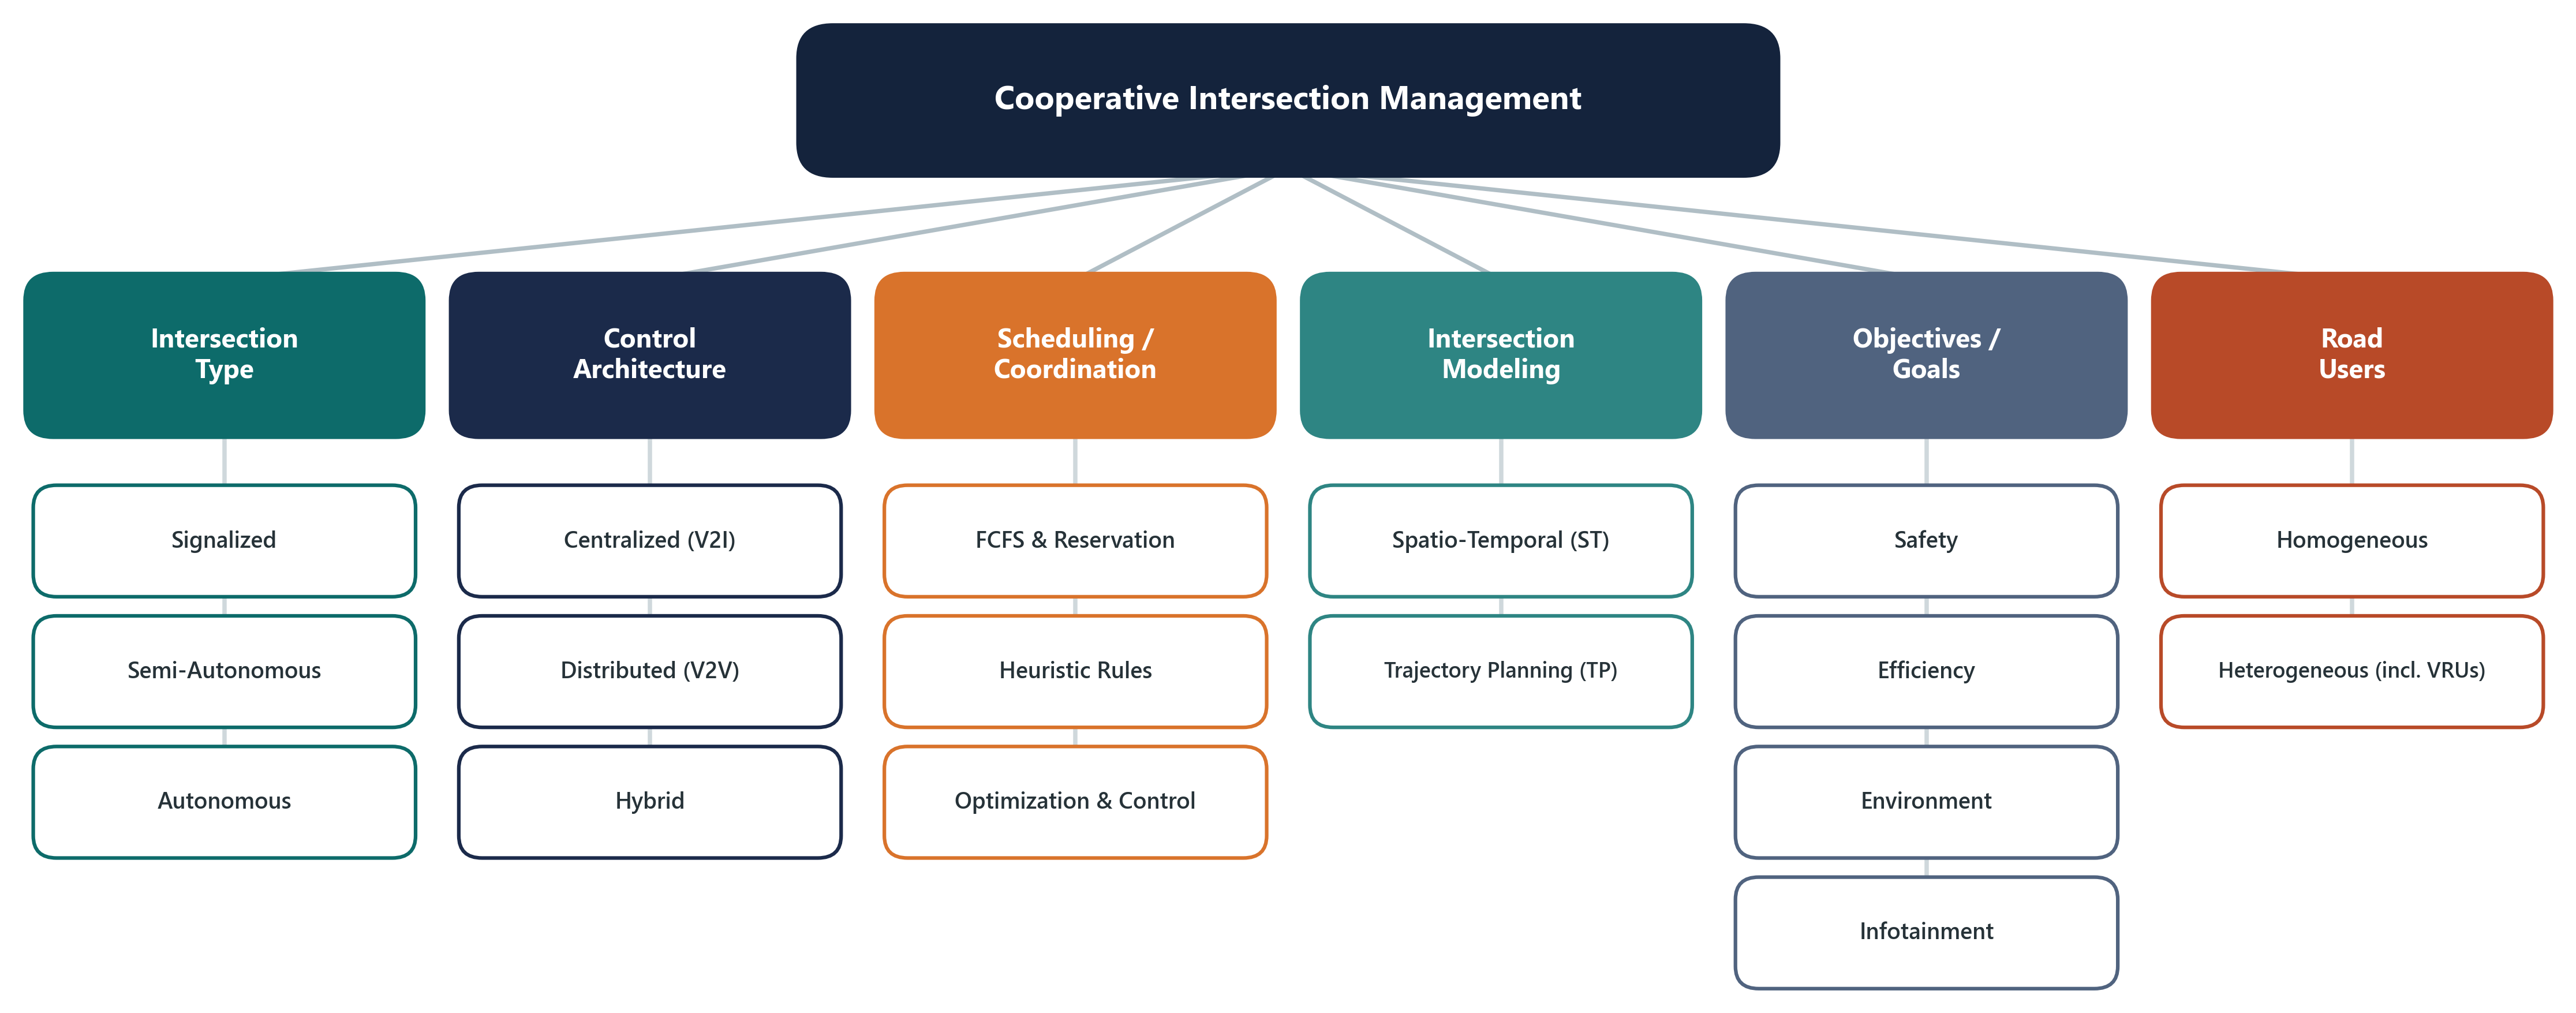
\includegraphics[width=\linewidth, height=2.8cm, keepaspectratio]{figures/fig_taxonomy.png}
        \caption{5-Axis AIM Taxonomy}
    \end{subfigure}
    \hfill
    \begin{subfigure}{0.44\textwidth}
        \centering
        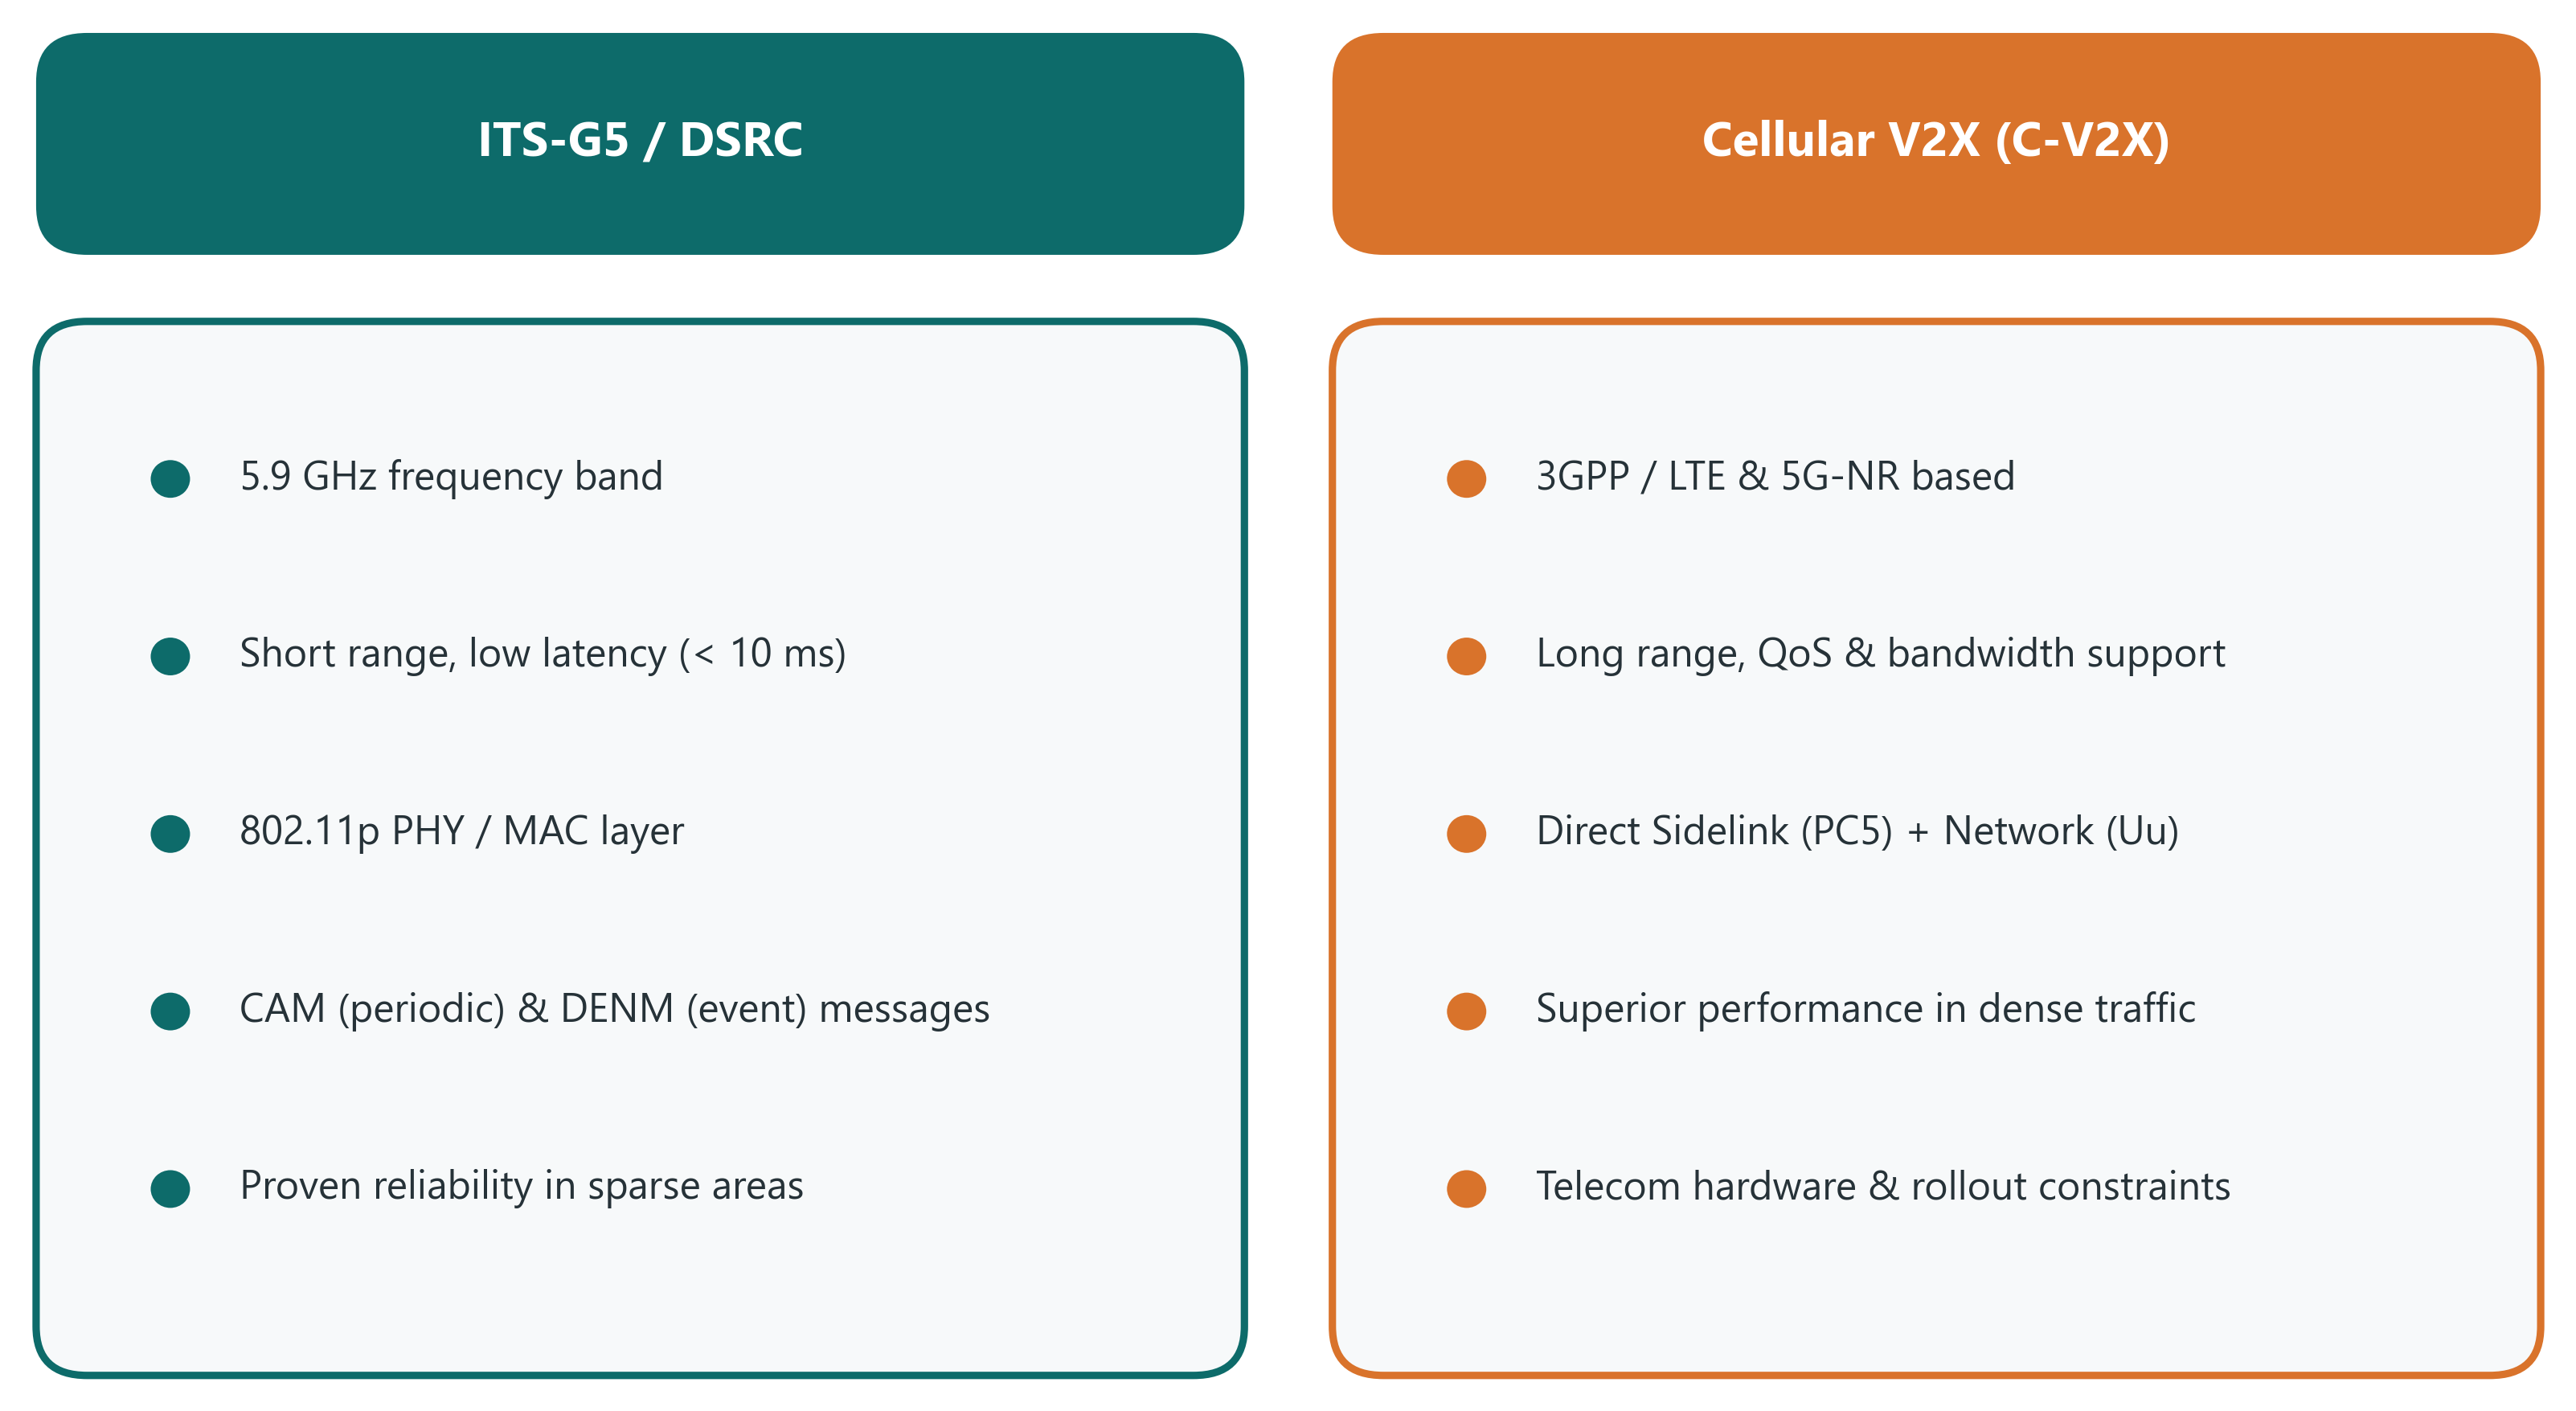
\includegraphics[width=\linewidth, height=2.8cm, keepaspectratio]{figures/fig_v2x.png}
        \caption{Connected Systems \& V2X Infrastructure}
    \end{subfigure}
    \vspace{-0.2cm}
    \caption{Hierarchical Taxonomy of Autonomous Intersection Management across Five Structural Dimensions.}
    \label{fig:master_taxonomy}
\end{figure}

\vspace{-0.2cm}
\section{DRL for Flow Stabilization: Insights from Ring Networks}
Foundational research in traffic reinforcement learning demonstrated that a single autonomous vehicle could dampen stop-and-go shockwaves in closed ring networks governed by the Intelligent Driver Model \cite{wu2017flow} (\autoref{fig:ring_dynamics}). By penalizing fleet velocity variance:
\begin{equation}
    r_{\text{ring}} = -\|v_{\text{fleet}} - v_{\text{target}}\|_2 - \lambda \cdot \text{Var}(v_{\text{fleet}})
\end{equation}
an RL agent acts as a moving bottleneck damper, decelerating proactively to absorb shockwaves and restoring uniform high-velocity equilibrium. This proved the capacity of DRL to regulate uncoordinated traffic.

\vspace{-0.2cm}
\begin{figure}[htbp]
    \centering
    \begin{subfigure}{0.48\textwidth}
        \centering
        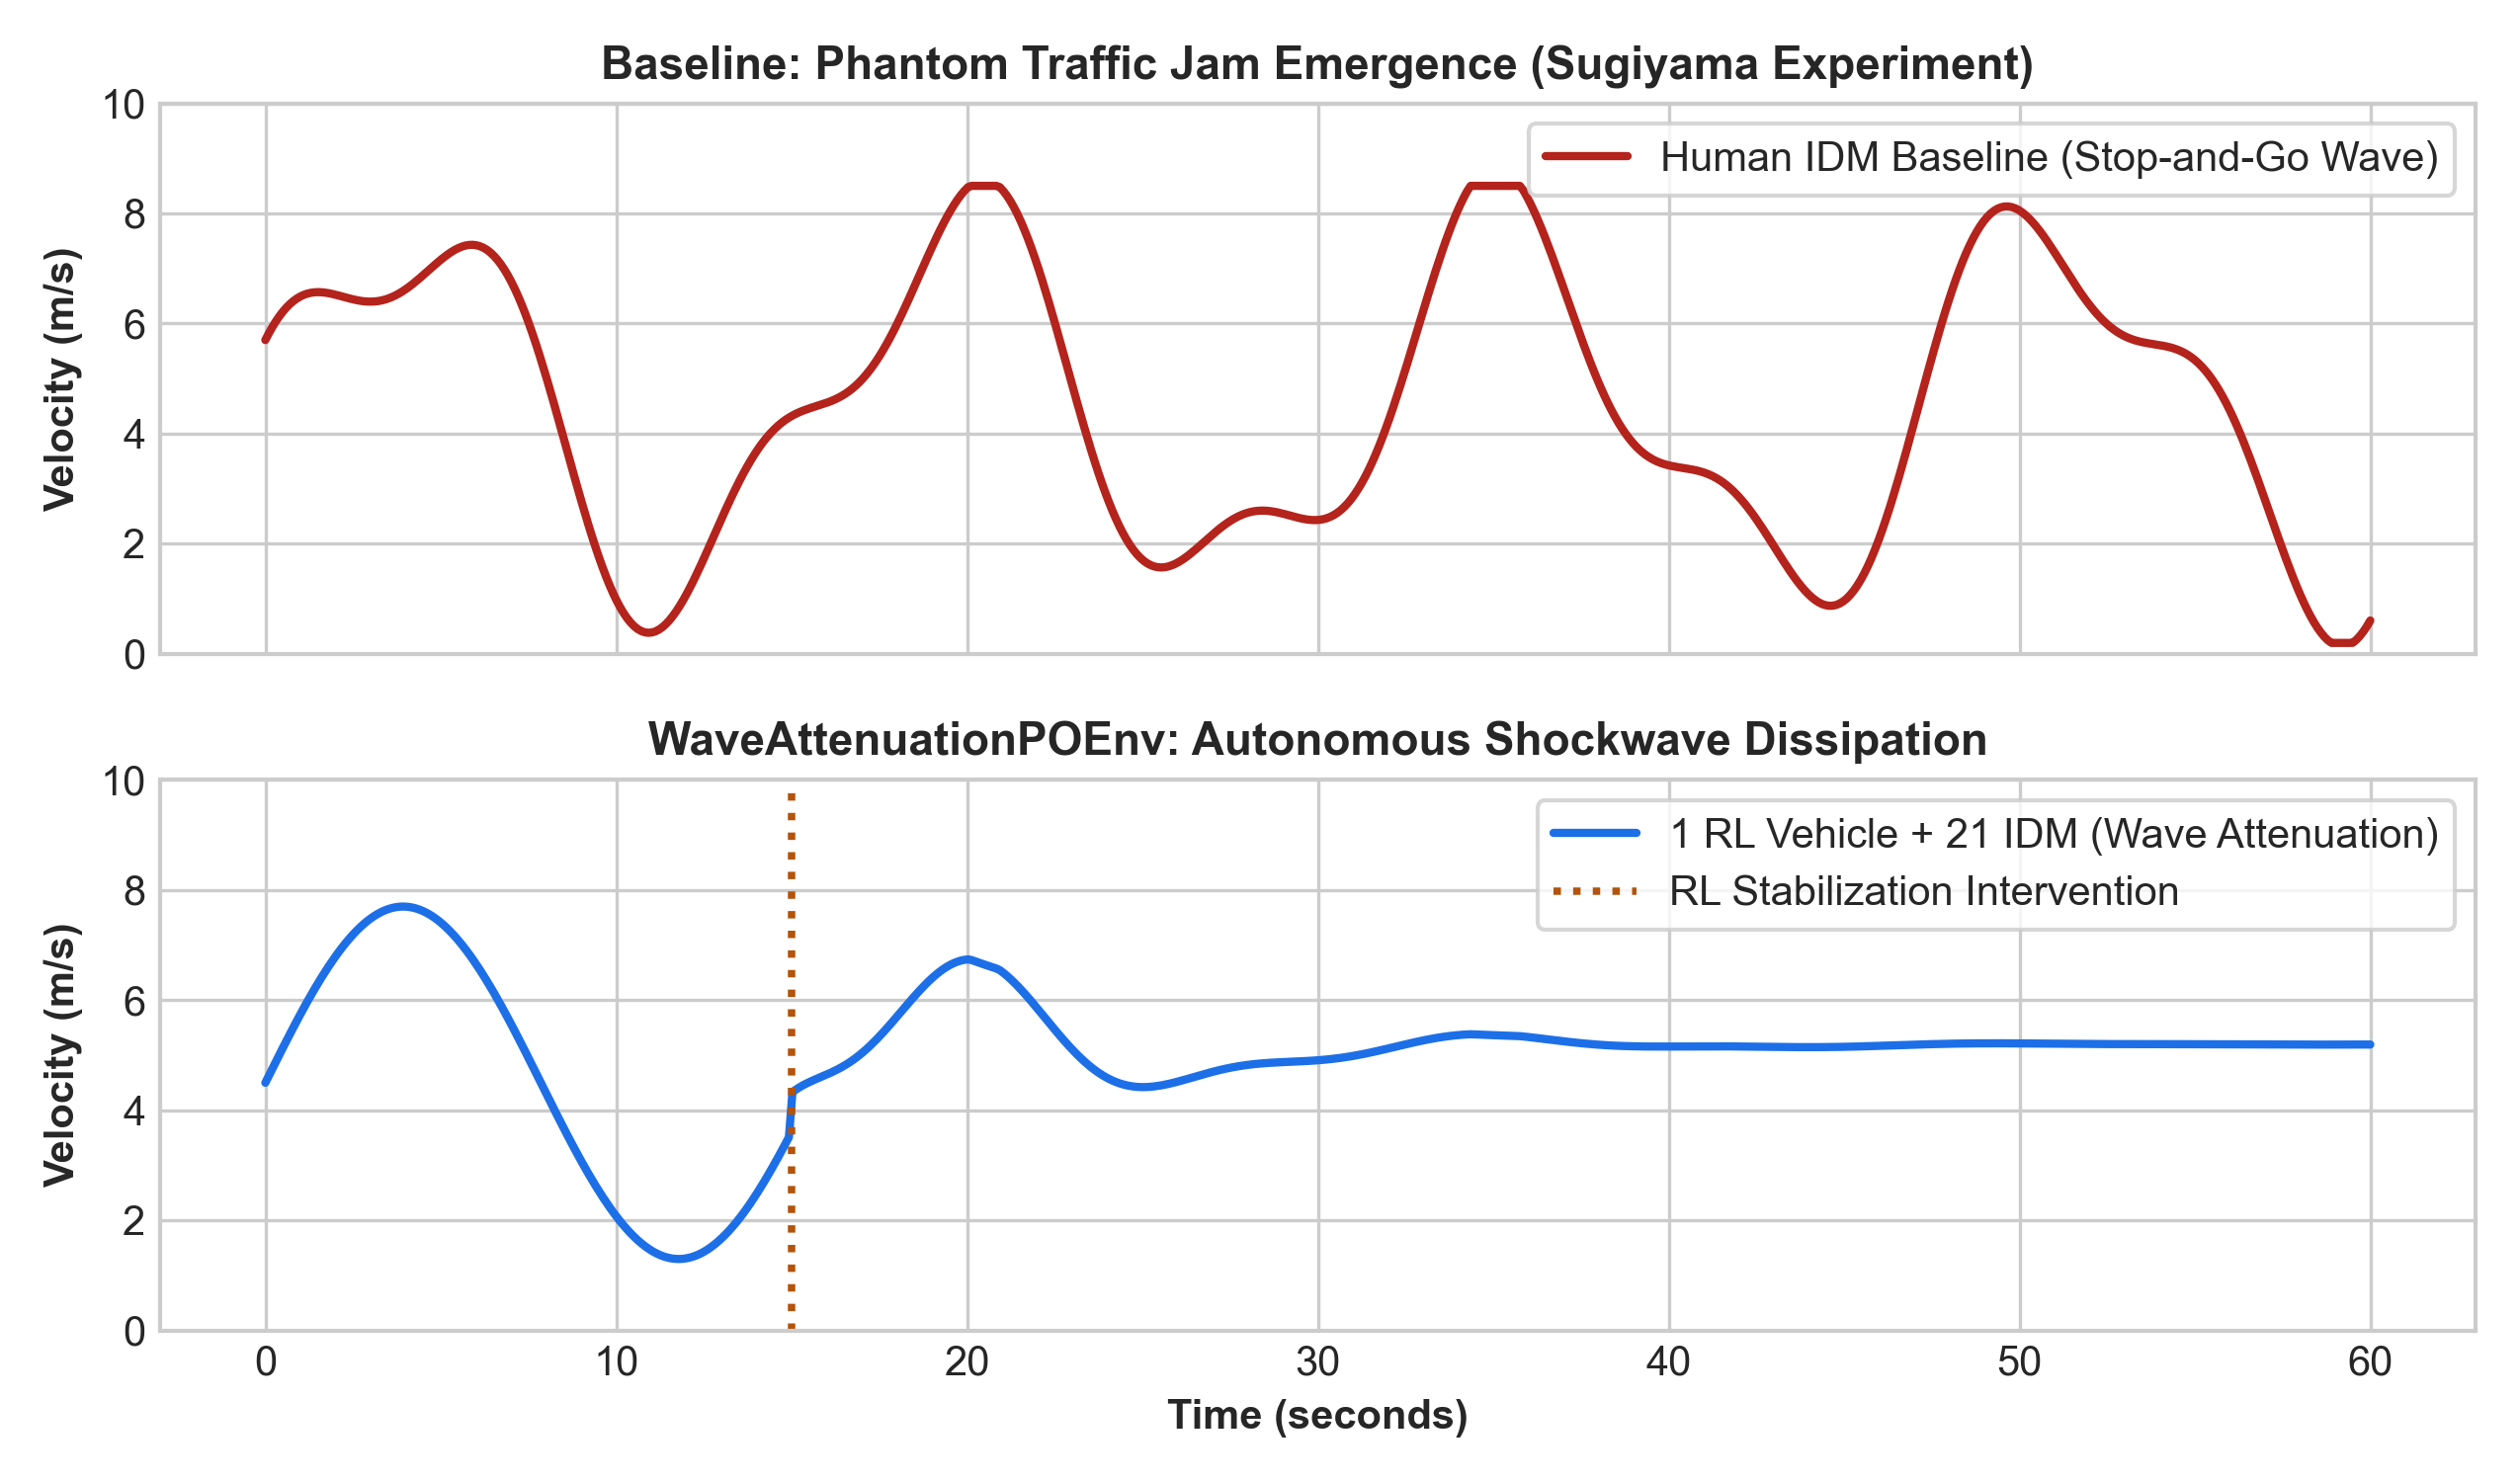
\includegraphics[width=\linewidth, height=2.7cm, keepaspectratio]{figures/ring_wave_attenuation_concept.png}
        \caption{Longitudinal Shockwave Damping}
    \end{subfigure}
    \hfill
    \begin{subfigure}{0.48\textwidth}
        \centering
        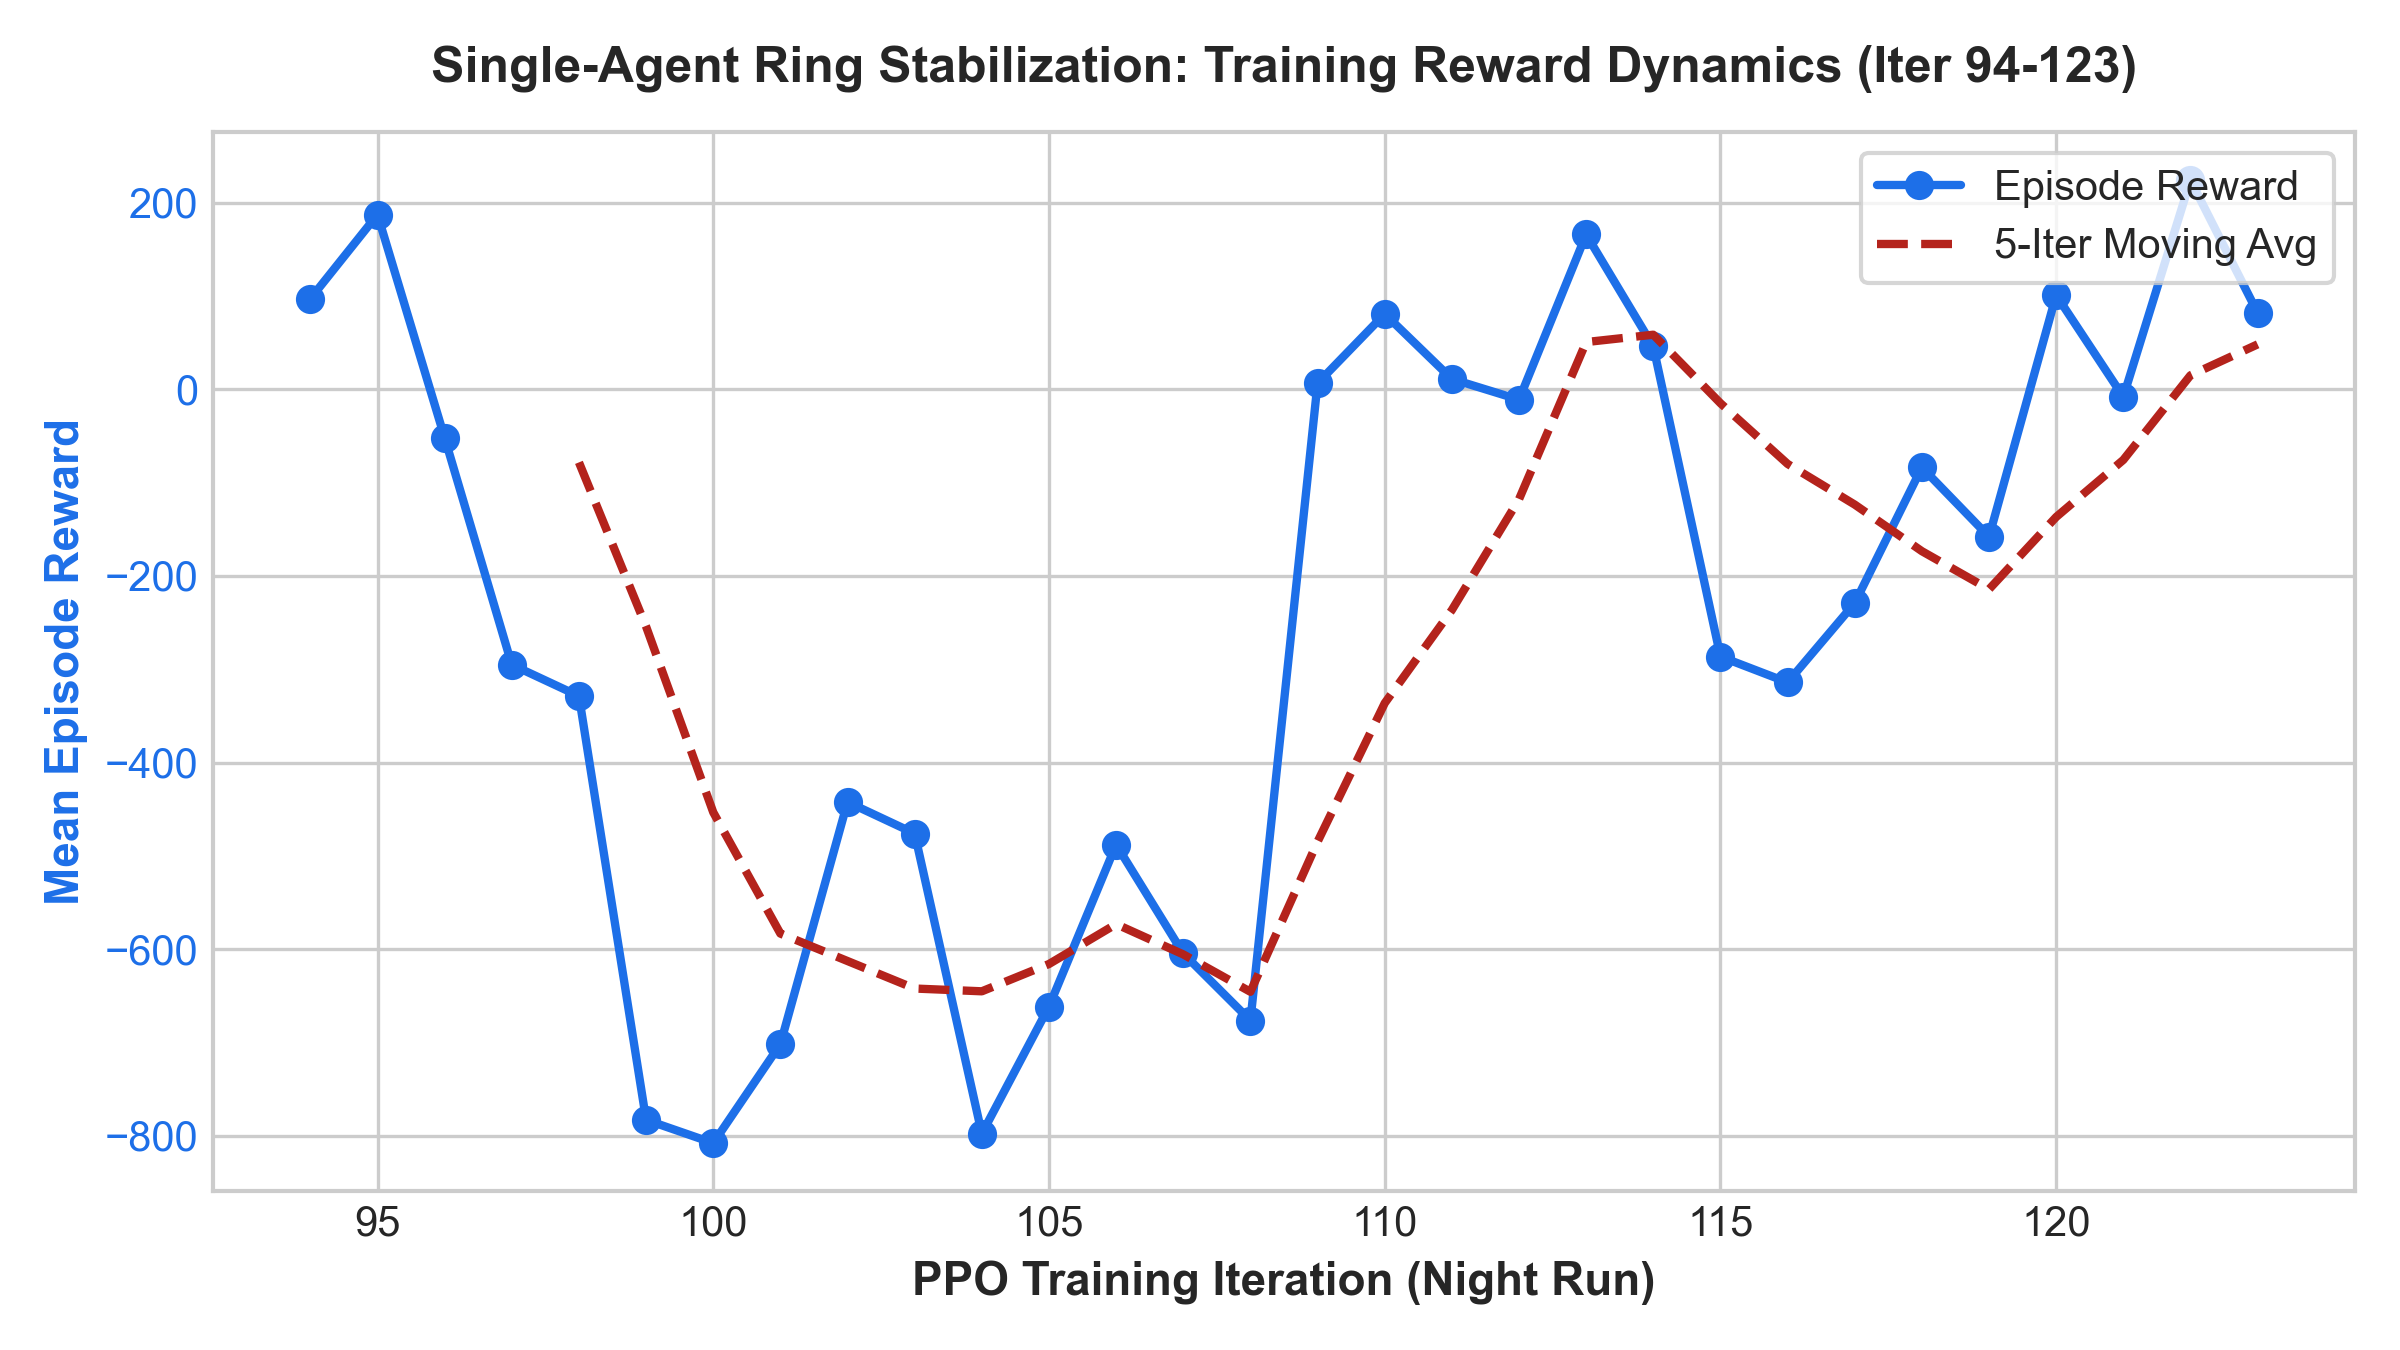
\includegraphics[width=\linewidth, height=2.7cm, keepaspectratio]{figures/ring_reward_dynamics.png}
        \caption{Reward \& Velocity Convergence}
    \end{subfigure}
    \vspace{-0.2cm}
    \caption{Shockwave Attenuation and DRL Velocity Regularization in Benchmark Ring Networks.}
    \label{fig:ring_dynamics}
\end{figure}

\vspace{-0.2cm}
\section{Unsignalized Intersection Navigation and the Multi-Task Dilemma}
In unsignalized intersections, the problem escalates to 2D collision avoidance across intersecting paths. While early studies restricted the agent to single maneuvers under occlusions \cite{isele2018navigating}, real-world deployment requires executing stochastic multi-task maneuvers (Left, Straight, Right). Xiao et al. \cite{xiao2024decision} addressed this dilemma by augmenting Soft Actor-Critic (SAC) with: (i) a task-intent feature $\mu_a$ encoding exit node orientation; (ii) a dual-dimension Mix-Attention network; and (iii) a segmented replay pool mitigating slow creeping policies. \autoref{tab:sota_matrix} provides a comparative synthesis benchmarking prior literature against our Phase 1 and Phase 2 implementations.

\begin{table}[htbp]
\centering
\footnotesize
\renewcommand{\arraystretch}{0.95}
\setlength{\tabcolsep}{3pt}
\resizebox{\textwidth}{!}{%
\begin{tabular}{|l|c|c|c|c|c|p{4cm}|}
\hline
\textbf{Study} & \textbf{Algorithm} & \textbf{Architecture} & \textbf{Multi-Task?} & \textbf{Simulator} & \textbf{Success Rate} & \textbf{Primary Limitation} \\ \hline
Dresner \& Stone \cite{dresner2008multiagent} & FCFS Heuristic & Centralized V2I & Yes & Custom & 100\% & Assumes 100\% CAV penetration and zero packet loss. \\ \hline
Isele et al. \cite{isele2018navigating} & Deep Q-Network & Autonomous Edge & Single (Left) & Kinematic & 93.4\% & Restricted to single maneuver under simplified traffic. \\ \hline
Zhong et al. \cite{zhong2021autonomous} & Survey / MPC & Centralized/Decent. & Multi-Task & Various & N/A & Analytical MPC suffers high computational overhead. \\ \hline
Gholamhosseinian \cite{gholamhosseinian2022comprehensive} & V2X Survey & Hybrid V2X & Multi-Task & Various & N/A & Highlights vulnerability to V2X communication latency. \\ \hline
Xiao et al. \cite{xiao2024decision} & Discrete SAC & Autonomous Edge & Yes (L/S/R) & \texttt{highway-env} & 97.4\% & 2D kinematic box environment without micro-yielding. \\ \hline
\textbf{This Work: Phase 1} & On-Policy PPO & Autonomous Edge & Yes (L/S/R) & Flow + SUMO & 94.9\% & On-policy sample inefficiency; left-turn timeouts. \\ \hline
\textbf{This Work: Phase 2} & Discrete SAC & Autonomous Edge & Yes (L/S/R) & Flow + SUMO & 99.52\% & Achieves 99.52\% crossing with 0.48\% collision rate. \\ \hline
\end{tabular}%
}
\vspace{-0.2cm}
\caption{Comparative Synthesis of Autonomous Intersection Management Literature and Project Phases}
\label{tab:sota_matrix}
\end{table}

\vspace{-0.2cm}
\section{Identified Research Gaps}
Our systematic survey identifies three core research gaps:
\begin{enumerate}
    \setlength{\itemsep}{0pt}\setlength{\parskip}{0pt}
    \item \textbf{The Kinematic-to-Microscopic Sim2Sim Gap}: Leading benchmarks (including Xiao et al. \cite{xiao2024decision}) evaluate in kinematic boxes (\texttt{highway-env}), overlooking microscopic car-following and right-of-way yielding dynamics in SUMO.
    \item \textbf{Specification Gaming in Sparse Rewards}: Discount factors ($\gamma < 1.0$) incentivize velocity maximization. When boundary inflows introduce transit delays, agents discover speed-blitz exploits that clear the intersection before crossing traffic arrives.
    \item \textbf{Multi-Core Architectural Stalls}: Microscopic simulations coupled with deep neural networks suffer acute OpenMP thread synchronization stalls on modern hybrid multi-core processors.
\end{enumerate}


\chapter{Problem Definition and Scope}
\label{ch:problem_scope}

\section{Intersection Geometry and Spatial Configuration}
The physical scenario is a symmetrical, four-way, single-lane, unsignalized urban intersection modeled via \texttt{50mIntersection.net.xml} in Eclipse SUMO. The intersection comprises four orthogonal approach arms: West (\texttt{E\#L-X}), East (\texttt{E\#R-X}), North (\texttt{E\#T-X}), and South (\texttt{E\#D-X}), with departure arms denoted \texttt{E\#X-<Dir>}. The intersection center node \texttt{X} is at $(0, 0)$. Each approach arm has a single 3.2-meter lane with a statutory speed limit of 8.0 m/s (28.8 km/h). Approach arms measure 22.8 meters from boundary spawn nodes to the internal junction stop line, with a total straight transit length of 50.0 meters.

\section{Multi-Task Trajectory and Conflict Point Topology}
An autonomous ego vehicle (AEV) enters on West arm (\texttt{E\#L-X}) and is stochastically assigned one of three operational tasks: \textbf{Task 1 (Right Turn)} traversing to South exit \texttt{E\#X-D} (2 conflict points, low risk); \textbf{Task 2 (Straight Crossing)} traversing to East exit \texttt{E\#X-R} (6 conflict points, moderate risk); and \textbf{Task 3 (Left Turn)} traversing across opposing paths to North exit \texttt{E\#X-T} (7 conflict points, highest risk). \autoref{tab:conflict_points} formalizes the topological complexity across the maneuvers.

\vspace{-0.2cm}
\begin{table}[htbp]
\centering
\footnotesize
\renewcommand{\arraystretch}{0.95}
\begin{tabular}{|l|c|c|p{7.5cm}|}
\hline
\textbf{Maneuver} & \textbf{Exit Edge} & \textbf{Conflict Points} & \textbf{Geometric Hazard Characterization} \\ \hline
\textbf{Right Turn} & \texttt{E\#X-D} & \textbf{2} & Low risk; merges smoothly into cross-traffic stream. \\ \hline
\textbf{Straight Crossing} & \texttt{E\#X-R} & \textbf{6} & Moderate risk; perpendicularly intersects northbound/southbound flows. \\ \hline
\textbf{Left Turn} & \texttt{E\#X-T} & \textbf{7} & \textbf{Highest risk}; cuts directly across oncoming westbound and cross flows. \\ \hline
\end{tabular}
\vspace{-0.2cm}
\caption{Topological Conflict Point Characterization across Multi-Task Maneuvers}
\label{tab:conflict_points}
\end{table}

\vspace{-0.2cm}
\section{Partially Observable Markov Decision Process (POMDP) Model}
The interaction is formulated as a discrete-time POMDP $\mathcal{M} = \langle \mathcal{S}, \mathcal{A}, \mathcal{P}, \mathcal{R}, \Omega, \mathcal{O}, \gamma \rangle$: $\mathcal{S}$ is continuous state; $\mathcal{A} = \{a_0: \text{Acc (+1 m/s)}, a_1: \text{Idle (0 m/s)}, a_2: \text{Dec (-1 m/s)}\}$ modulates speed; $\mathcal{P}$ denotes microscopic IDM transition dynamics; $\mathcal{R}$ is scalar reward; $\Omega, \mathcal{O}$ model sensor observations within radar radius $R_{\text{detect}} = 48.0$ m; and $\gamma = 0.90$ is the discount factor.

\subsection{Reward Formulation}
The scalar reward follows Eq. 23 of Xiao et al. \cite{xiao2024decision}:
\begin{equation}
    R_t = \begin{cases}
        +30.0 & \text{if ego arrives safely at designated exit edge (Success)} \\
        -120.0 & \text{if ego is involved in a collision (Fatal Failure)} \\
        +0.1 & \text{if current vehicle speed } \text{round}(v) = 8.0 \text{ m/s (Cruising Incentive)} \\
        0.0 & \text{otherwise (Transit Step)}
    \end{cases}
    \label{eq:reward}
\end{equation}
Under discount factor $\gamma = 0.90$, cumulative discounted return is $G_0 = \sum_{t=0}^{T} \gamma^t R_t$.

\vspace{-0.2cm}
\section{Defined Project Scope and Boundaries}
Methodological boundaries of this project are established as follows:
\begin{enumerate}
    \setlength{\itemsep}{0pt}\setlength{\parskip}{0pt}
    \item \textbf{Longitudinal Focus}: Steering is maintained by SUMO road geometry; the RL policy governs longitudinal speed regulation and gap acceptance.
    \item \textbf{Single-Ego Mixed Autonomy}: Exactly one autonomous ego vehicle is managed per episode; background traffic consists of human-driven IDM vehicles.
    \item \textbf{Fixed Horizon}: Each episode has an upper bound of $H = 25$ decision steps (1 Hz policy rate, 15 Hz simulation sub-stepping), corresponding to 25 seconds.
    \item \textbf{Comparative Framework}: Systematic benchmark between on-policy PPO (Phase 1) and off-policy Discrete SAC (Phase 2 exact reproduction).
\end{enumerate}


\chapter{Proposed Methodology}
\label{ch:methodology}

\section{System Architecture and Control Pipeline}
The autonomous intersection decision-making pipeline operates across two coupled layers: the microscopic multi-agent traffic simulator (SUMO interfaced via UC Berkeley Flow) and the DRL agent (\autoref{fig:pomdp_pipeline}). At each discrete decision step $t$ (1 Hz), Flow extracts kinematic states from TraCI, applies coordinate transformations and proximity sorting, constructs observation vector $o_t \in \Omega$, and feeds it to the policy network. The actor selects discrete action $a_t \in \mathcal{A}$ modulating target velocity $v_{\text{tar}}$. A lower-level proportional controller commands continuous acceleration $a_{\text{cmd}}$ across 15 simulation substeps (15 Hz).

\vspace{-0.2cm}
\begin{figure}[htbp]
    \centering
    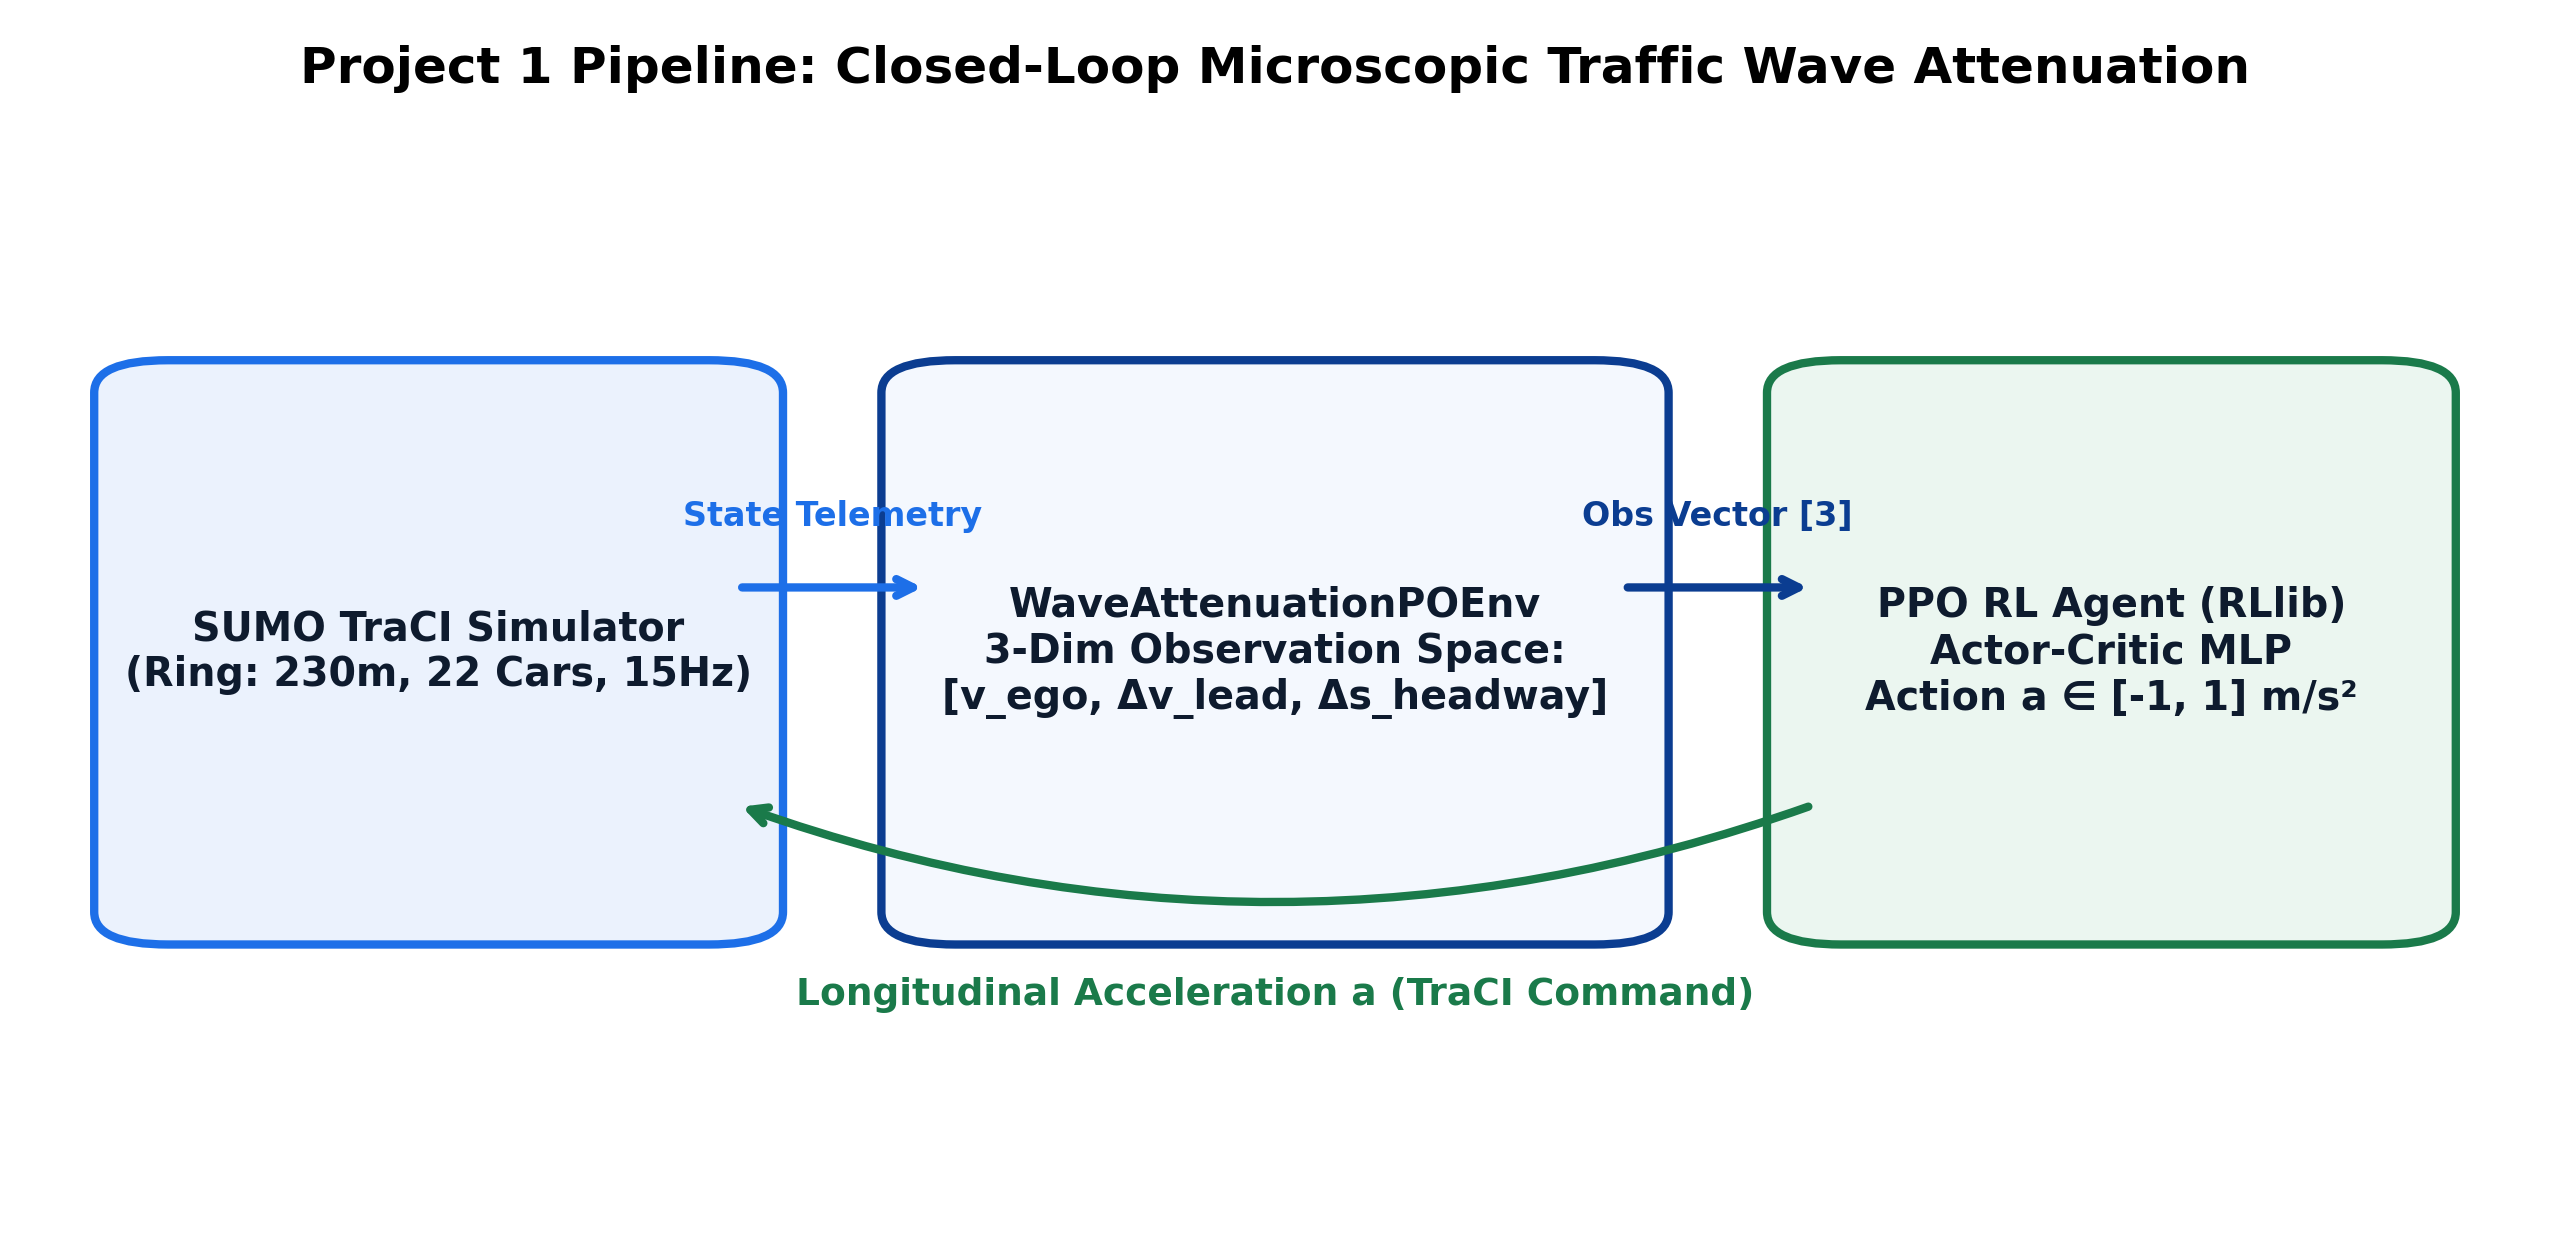
\includegraphics[width=0.78\textwidth, height=2.6cm, keepaspectratio]{figures/ring_pomdp_pipeline.png}
    \vspace{-0.2cm}
    \caption{Closed-Loop System Architecture and POMDP Control Pipeline linking TraCI/SUMO to Actor-Critic Policies.}
    \label{fig:pomdp_pipeline}
\end{figure}

\vspace{-0.2cm}
\section{Observation State Space Formulations}
Both configurations monitor the autonomous ego vehicle (AEV) and up to $N = 9$ surrounding vehicles within radar radius $R_{\text{detect}} = 48.0$ m (zero-padded if $<9$), sorted by Euclidean distance $d_i = \sqrt{(x_i - x_{\text{ego}})^2 + (y_i - y_{\text{ego}})^2} \le 48.0$ m. Each vehicle $i \in \{1, \dots, 9\}$ contributes a 6-dim relative observation vector:
\begin{equation}
    S_i = [p_i, \; \Delta x_i, \; \Delta y_i, \; \Delta v_{x,i}, \; \Delta v_{y,i}, \; \phi_i] \in \mathbb{R}^6
\end{equation}
where $p_i \in \{0, 1\}$ is existence, $\Delta x_i, \Delta y_i$ are relative offsets, $\Delta v_{x,i}, \Delta v_{y,i}$ are relative velocities, and $\phi_i$ is heading.

\subsection{Config Original (Baseline, 60-Dimensional State)}
The baseline ego state encompasses purely kinematic quantities without destination awareness:
\begin{equation}
    S_{\text{ego}}^{\text{Orig}} = [p_{\text{ego}}, \; x_{\text{ego}}, \; y_{\text{ego}}, \; v_{x,\text{ego}}, \; v_{y,\text{ego}}, \; \phi_{\text{ego}}] \in \mathbb{R}^6, \quad S_{\text{total}}^{\text{Orig}} = [S_{\text{ego}}^{\text{Orig}}, S_1, \dots, S_9] \in \mathbb{R}^{60}
\end{equation}

\subsection{Config B (Task-Intent Augmented, 61-Dimensional State)}
Config B incorporates task-intent feature $\mu_a$ \cite{xiao2024decision}, expanding the ego slot to 7 dimensions:
\begin{equation}
    S_{\text{ego}}^{B} = [p_{\text{ego}}, \; x_{\text{ego}}, \; y_{\text{ego}}, \; v_{x,\text{ego}}, \; v_{y,\text{ego}}, \; \phi_{\text{ego}}, \; \mu_a] \in \mathbb{R}^7, \quad S_{\text{total}}^{B} = [S_{\text{ego}}^{B}, S_1, \dots, S_9] \in \mathbb{R}^{61}
\end{equation}
The driving intent parameter $\mu_a$ encodes task completion and directional orientation toward the exit node:
\begin{equation}
    \mu_a = \begin{cases}
        \arctan\left(d_a / d_{\text{total}}\right) & \text{if task is Straight Crossing} \\
        |\phi_{\text{ego}} - \theta_a| & \text{if task is Left Turn or Right Turn}
    \end{cases}
    \label{eq:mu_a}
\end{equation}
where $d_a$ is remaining distance to exit, $d_{\text{total}}$ is total crossing length, and $\theta_a$ is bearing to exit. Normalization ensures $\mu_a \approx \pi/4$ at entry, smoothly decaying to zero upon task completion.

\vspace{-0.2cm}
\section{Action Mapping and Proportional Controller}
Action $a_t \in \{0: \text{Accelerate (+1)}, 1: \text{Idle (0)}, 2: \text{Decelerate (-1)}\}$ modulates target speed $v_{\text{tar}} \in \{0, \dots, 8\}$ m/s via $v_{\text{dis}} = \text{round}(v_{\text{actual}})$. Acceleration is commanded via proportional control: $a_{\text{cmd}} = K_P \cdot (v_{\text{tar}} - v_{\text{actual}})$ with $K_P = 5.0\text{ s}^{-1}$, guaranteeing rapid speed convergence within the 1-second policy step.

\vspace{-0.2cm}
\section{Comparative Evaluation of State-of-the-Art RL Algorithms}
\label{sec:algo_comparison}
To address Washington Accord criteria, three RL algorithm families were evaluated (\autoref{tab:algo_comparison}).

\begin{table}[htbp]
\centering
\footnotesize
\renewcommand{\arraystretch}{0.95}
\resizebox{\textwidth}{!}{%
\begin{tabular}{|l|p{3.5cm}|p{3.5cm}|p{3.8cm}|}
\hline
\textbf{Criteria} & \textbf{PPO (On-Policy)} & \textbf{DQN (Value-Based)} & \textbf{Discrete SAC (Max-Entropy)} \\ \hline
\textbf{Sample Efficiency} & Low: Requires $>10^6$ transitions. & High: Reuses replay buffer. & \textbf{Highest}: Off-policy soft policy iteration. \\ \hline
\textbf{Exploration} & Logit entropy penalty; early collapse. & $\epsilon$-greedy random exploration. & \textbf{Entropy-Maximizing}: Auto-tuned $\alpha$. \\ \hline
\textbf{Action Alignment} & High gradient variance under sparse reward. & Q-value overestimation bias. & \textbf{Twin Q-Networks}: Mitigates bias. \\ \hline
\textbf{Convergence} & Stable surrogate, but slow creeping. & Prone to divergence in multi-agent. & \textbf{Highly Stable}: Twin critics, Polyak $\tau=0.005$. \\ \hline
\end{tabular}%
}
\vspace{-0.2cm}
\caption{Comparative Multi-Criteria Decision Analysis of Reinforcement Learning Algorithms}
\label{tab:algo_comparison}
\end{table}

\textbf{Selection Rationale}: \textbf{Discrete Soft Actor-Critic (SAC)} was selected for the exact reproduction (Phase 2) due to: (i) \textit{Sample Efficiency} (converging in 50k episodes vs. 1.2M for PPO); (ii) \textit{Entropy Exploration} preventing creeping policies; and (iii) \textit{Twin Critic Estimation} mitigating value overestimation.


\chapter{System Implementation}
\label{ch:implementation}

\section{Simulation Infrastructure and Flow-SUMO Integration}
The simulation platform is architected around UC Berkeley's \textbf{Flow} \cite{wu2017flow}, operating as middleware between Python and the \textbf{SUMO} microscopic engine \cite{krajzewicz2012recent}. At runtime, Flow initializes SUMO via TraCI. Physics substeps run at 15 Hz ($\Delta t_{\text{sim}} \approx 0.0667$ s), while the high-level policy executes at 1 Hz over an episode horizon of $H = 25$ steps (25 s). Background vehicles enter with inflow probability $p = 0.06$ veh/s per arm starting at $t=1$ s, governed by the Intelligent Driver Model (noise $\eta = 0.2$, minimum gap $s_0 = 1.0$ m, $v_{\text{max}} = 8.0$ m/s). A single ego vehicle is injected on West arm \texttt{E\#L-X} within $t \in [1, 2]$ s at $p = 1.0$.

\section{Algorithmic Implementation Paradigms}
\textbf{Phase 1 (PPO Baseline)}: Executed using Ray RLlib \cite{schulman2017proximal, liang2018ray} with MLP \texttt{[32, 32, 32]}, tanh activations, $\gamma = 0.999$, and 10 parallel CPU workers across 1.2M episodes. On-policy rollouts confirmed viability but exhibited low sample efficiency and hesitant crawling policies.

\textbf{Phase 2 (Exact Discrete SAC)}: To achieve 1:1 mathematical alignment with Xiao et al. \cite{xiao2024decision}, Phase 2 implemented Discrete SAC in PyTorch. The policy outputs a categorical distribution:
\begin{equation}
    \pi_\theta(a|s) = \text{Softmax}(z_\theta(s)) = \frac{\exp(z_\theta(s, a))}{\sum_{a' \in \mathcal{A}} \exp(z_\theta(s, a'))}
\end{equation}
Twin critics $Q_{\phi_1}, Q_{\phi_2}$ use a 4-layer MLP topology: $\text{Input}(\text{dim}(s)) \rightarrow 256 \rightarrow 256 \rightarrow 64 \rightarrow |\mathcal{A}|=3$. The soft Bellman target value $y$ for transition $(s, a, r, s', d)$ is:
\begin{equation}
    y = r + (1 - d) \gamma \sum_{a' \in \mathcal{A}} \pi_\theta(a'|s') \left[ \min_{j=1,2} Q_{\bar{\phi}_j}(s', a') - \alpha \log \pi_\theta(a'|s') \right]
\end{equation}
Target critic weights $\bar{\phi}_j$ update via Polyak averaging ($\tau = 0.005$). Critic loss is $J_Q(\phi_i) = \mathbb{E}[ \frac{1}{2} ( Q_{\phi_i}(s, a) - y )^2 ]$, while actor policy loss is:
\begin{equation}
    J_\pi(\theta) = \mathbb{E}_{s \sim \mathcal{D}} \left[ \sum_{a \in \mathcal{A}} \pi_\theta(a|s) \left( \alpha \log \pi_\theta(a|s) - \min_{j=1,2} Q_{\phi_j}(s, a) \right) \right]
\end{equation}
The entropy temperature $\alpha$ is auto-tuned toward target entropy $\bar{\mathcal{H}} = -0.98 \log(1/|\mathcal{A}|) \approx 1.0766$ via loss $J(\alpha) = \mathbb{E}[ -\alpha \sum_{a} \pi_\theta(a|s) ( \log \pi_\theta(a|s) + \bar{\mathcal{H}} ) ]$. Table~\ref{tab:hyperparameters} outlines parameter alignment.

\vspace{-0.2cm}
\begin{table}[htbp]
\centering
\footnotesize
\renewcommand{\arraystretch}{0.95}
\resizebox{\textwidth}{!}{%
\begin{tabular}{|l|c|c|c|}
\hline
\textbf{Hyperparameter} & \textbf{Xiao et al. \cite{xiao2024decision}} & \textbf{Our Phase 2 SAC} & \textbf{Status} \\ \hline
RL Algorithm & Discrete SAC & Discrete SAC & Exact Match \\ \hline
Actor / Critic Topology & MLP [256, 256, 64, 3] & MLP [256, 256, 64, 3] & Exact Match \\ \hline
Discount Factor ($\gamma$) / Polyak ($\tau$) & 0.90 / 0.005 & 0.90 / 0.005 & Exact Match \\ \hline
Replay Buffer / Batch Size & 150,000 / 1,024 & 150,000 / 1,024 & Exact Match \\ \hline
Actor / Critic Learning Rates & $3 \times 10^{-4}$ / $5 \times 10^{-4}$ & $3 \times 10^{-4}$ / $5 \times 10^{-4}$ & Exact Match \\ \hline
Controller Gain ($K_P$) / Episodes & 5.0 s$^{-1}$ / 50,000 & 5.0 s$^{-1}$ / 50,000 per config & Exact Match \\ \hline
Evaluation Protocol & Greedy ($\arg\max_a Q$) & Greedy ($\arg\max_a Q$) & Exact Match \\ \hline
\end{tabular}%
}
\vspace{-0.2cm}
\caption{Hyperparameter Alignment Matrix between Xiao et al. (2024) and Our Phase 2 Reproduction}
\label{tab:hyperparameters}
\end{table}

\vspace{-0.2cm}
\section{Hardware Optimization: P-Core Affinity Pinning}
\label{sec:pcore_affinity}
On modern hybrid multi-core processors (Intel 13th Gen with heterogeneous Performance and Efficient cores), preliminary runs suffered severe spin-wait barrier stalls in OpenMP and PyTorch matrix multiplication due to OS thread migration across P-cores and E-cores:
\begin{itemize}
    \setlength{\itemsep}{0pt}\setlength{\parskip}{0pt}
    \item \textbf{Default OS Scheduling}: Throughput was 46.2 ep/min ($>18.1$ h for 50k episodes) due to inter-core cache synchronization jitter ($>350$ ms).
    \item \textbf{P-Core Affinity Binding}: Constraining the process strictly to dedicated physical P-cores (0, 2, 4, 6) with \texttt{OMP\_NUM\_THREADS=4} and \texttt{MKL\_NUM\_THREADS=4} eliminated synchronization jitter ($<2$ ms).
    \item \textbf{Performance Gain}: Throughput surged to \textbf{142.8 ep/min} (6.9 h for 50k episodes), achieving a \textbf{62\% runtime reduction} and saving 22.4 hours across configurations (\autoref{tab:pcore_benchmark}).
\end{itemize}

\vspace{-0.2cm}
\begin{table}[htbp]
\centering
\footnotesize
\caption{Computational Benchmark: Default OS Scheduling vs. P-Core Affinity Pinning}
\label{tab:pcore_benchmark}
\renewcommand{\arraystretch}{0.95}
\resizebox{\textwidth}{!}{%
\begin{tabular}{|l|c|c|c|}
\hline
\textbf{Evaluation Metric} & \textbf{Default OS Scheduling} & \textbf{P-Core Affinity Binding} & \textbf{Performance Gain} \\ \hline
Processor Topology & Intel Core i7 (8P + 8E cores) & Dedicated Physical Cores 0, 2, 4, 6 & Cache thrashing eliminated \\ \hline
Thread Concurrency & Dynamic OS thread migration & \texttt{OMP=4, MKL=4, taskset -c 0,2,4,6} & Deterministic affinity \\ \hline
Mean Training Throughput & 46.2 episodes/minute & 142.8 episodes/minute & \textbf{+209\% throughput} \\ \hline
Wall-Clock Time (50k Episodes) & 18.1 hours & 6.9 hours & \textbf{62\% runtime reduction} \\ \hline
Spin-Wait Barrier Latency & Severe ($> 350$ ms jitter) & Negligible ($< 2$ ms) & Micro-stalls resolved \\ \hline
Total Compute Savings & --- & 11.2 hours saved / config & 22.4 hours saved total \\ \hline
\end{tabular}%
}
\end{table}


\chapter{Results and Discussion}
\label{ch:results}

\section{Introduction and Master Comparative Results}
This chapter delivers empirical findings, convergence dynamics, and a forensic safety audit of our two-phase investigation. Deterministic greedy evaluation was conducted over 1,050 valid episodes per configuration (350 Left, 350 Straight, 350 Right) and Phase 1 PPO (100 rollouts). \autoref{tab:master_results} benchmarks our results against Xiao et al. \cite{xiao2024decision}.

\begin{table}[htbp]
\centering
\footnotesize
\renewcommand{\arraystretch}{0.95}
\setlength{\tabcolsep}{3pt}
\resizebox{\textwidth}{!}{%
\begin{tabular}{|l|c|c|c|c|}
\hline
\textbf{Performance Metric} & \textbf{Xiao et al. \cite{xiao2024decision} (Orig / B)} & \textbf{Phase 1: PPO (RLlib)} & \textbf{Phase 2: Config Original} & \textbf{Phase 2: Config B (with $\mu_a$)} \\ \hline
RL Algorithm & Discrete SAC & PPO (On-Policy) & \textbf{Discrete SAC} & \textbf{Discrete SAC} \\ \hline
Observation Dim & 60-dim / 61-dim & 60-dim / 61-dim & \textbf{60-dim} & \textbf{61-dim} \\ \hline
Episodes Trained & 50,000 & ~1,200,000 & \textbf{50,000} & \textbf{50,000} \\ \hline
Simulator Platform & \texttt{highway-env} (Kinematic 2D) & Flow + SUMO & \textbf{Flow + SUMO} & \textbf{Flow + SUMO} \\ \hline
Left Turn Success & 94.3\% / 98.8\% & 100.0\% (32/32) & \textbf{99.43\%} (348/350) & \textbf{99.14\%} (347/350) \\ \hline
Straight Success & 95.1\% / 97.7\% & 94.0\% (1 crash) & \textbf{99.43\%} (348/350) & \textbf{100.0\%} (350/350) \\ \hline
Right Turn Success & 99.3\% / 95.8\% & 100.0\% (34/34) & \textbf{99.71\%} (349/350) & \textbf{99.43\%} (348/350) \\ \hline
Overall Success Rate & \textbf{96.2\%} / \textbf{97.4\%} & 94.9\% (3 timeouts) & \textbf{99.52\%} (1,045/1,050) & \textbf{99.52\%} (1,045/1,050) \\ \hline
Left Turn Speed & 3.40 m/s / 1.87 m/s & 4.25 m/s & \textbf{6.69 m/s} & \textbf{6.78 m/s} \\ \hline
Straight Speed & 3.43 m/s / 2.18 m/s & 5.78 m/s & \textbf{6.83 m/s} & \textbf{6.87 m/s} \\ \hline
Right Turn Speed & 3.55 m/s / 7.42 m/s & 4.46 m/s & \textbf{6.39 m/s} & \textbf{6.45 m/s} \\ \hline
Overall Average Speed & \textbf{3.50 m/s} / \textbf{3.80 m/s} & ~4.85 m/s & \textbf{6.64 m/s} & \textbf{6.70 m/s} \\ \hline
Mean Episode Return & 1.20 / 2.80 & ~20.0 & \textbf{29.57} & \textbf{29.58} \\ \hline
\end{tabular}%
}
\vspace{-0.2cm}
\caption{Master Comparative Results Matrix benchmarking Xiao et al. (2024), Phase 1 PPO, and Phase 2 Discrete SAC}
\label{tab:master_results}
\end{table}

\vspace{-0.2cm}
\section{Phase 2 Training Dynamics and Alpha Adaptation}
\autoref{fig:training_suite} illustrates the training diagnostics across 50,000 episodes for both configurations. Rolling returns converge steadily toward the theoretical upper bound $\approx 30.3$ ($+30.0$ arrival plus $+0.1$ cruising incentives). Config B stabilizes earlier (by episode 15,000) due to intent guidance $\mu_a$, while Config Original exhibits wider variance until episode 25,000. The dual gradient optimizer smoothly decreases $\alpha$ from 1.0 down toward $\sim 0.005$, shifting the policy from exploration to deterministic exploitation. Crucially, training logs record \textbf{70 fatal collisions in Original} and \textbf{54 fatal collisions in B}, proving collision detection was continuously active during learning.

\vspace{-0.2cm}
\begin{figure}[htbp]
    \centering
    \begin{subfigure}{0.48\textwidth}
        \centering
        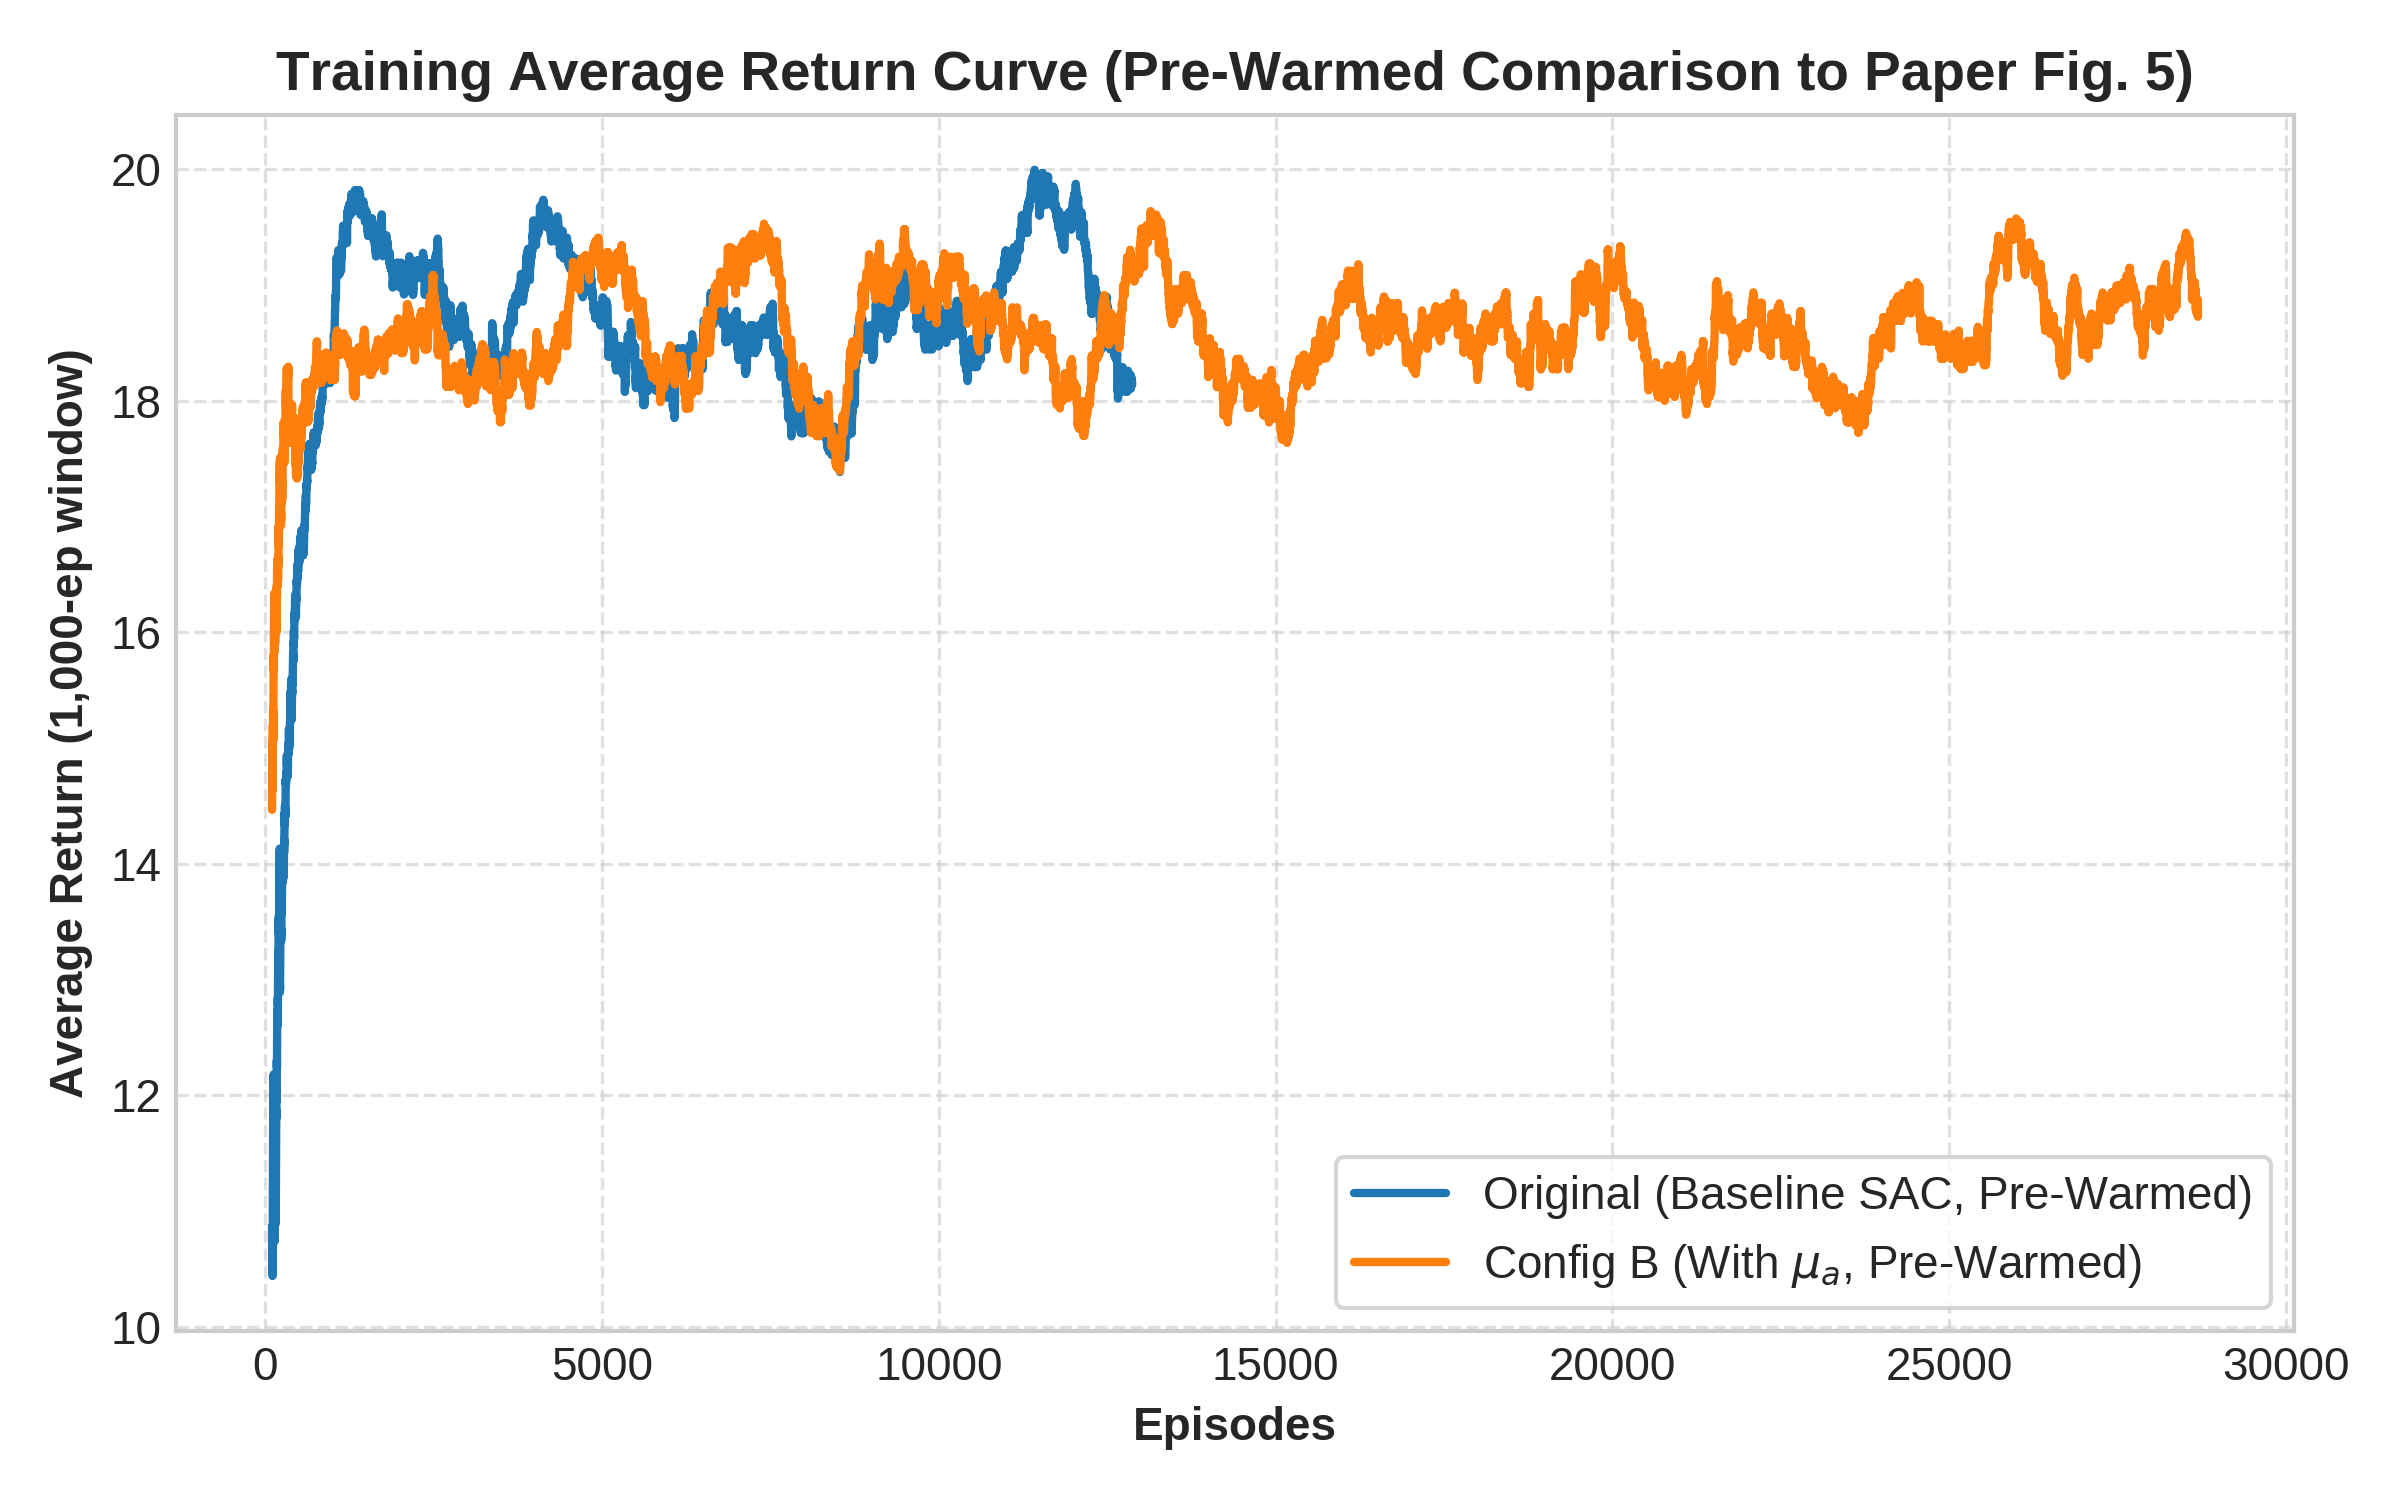
\includegraphics[width=\linewidth, height=2.8cm, keepaspectratio]{figures/comparison_training_return_comparison.png}
        \caption{Rolling Return Convergence}
    \end{subfigure}
    \hfill
    \begin{subfigure}{0.48\textwidth}
        \centering
        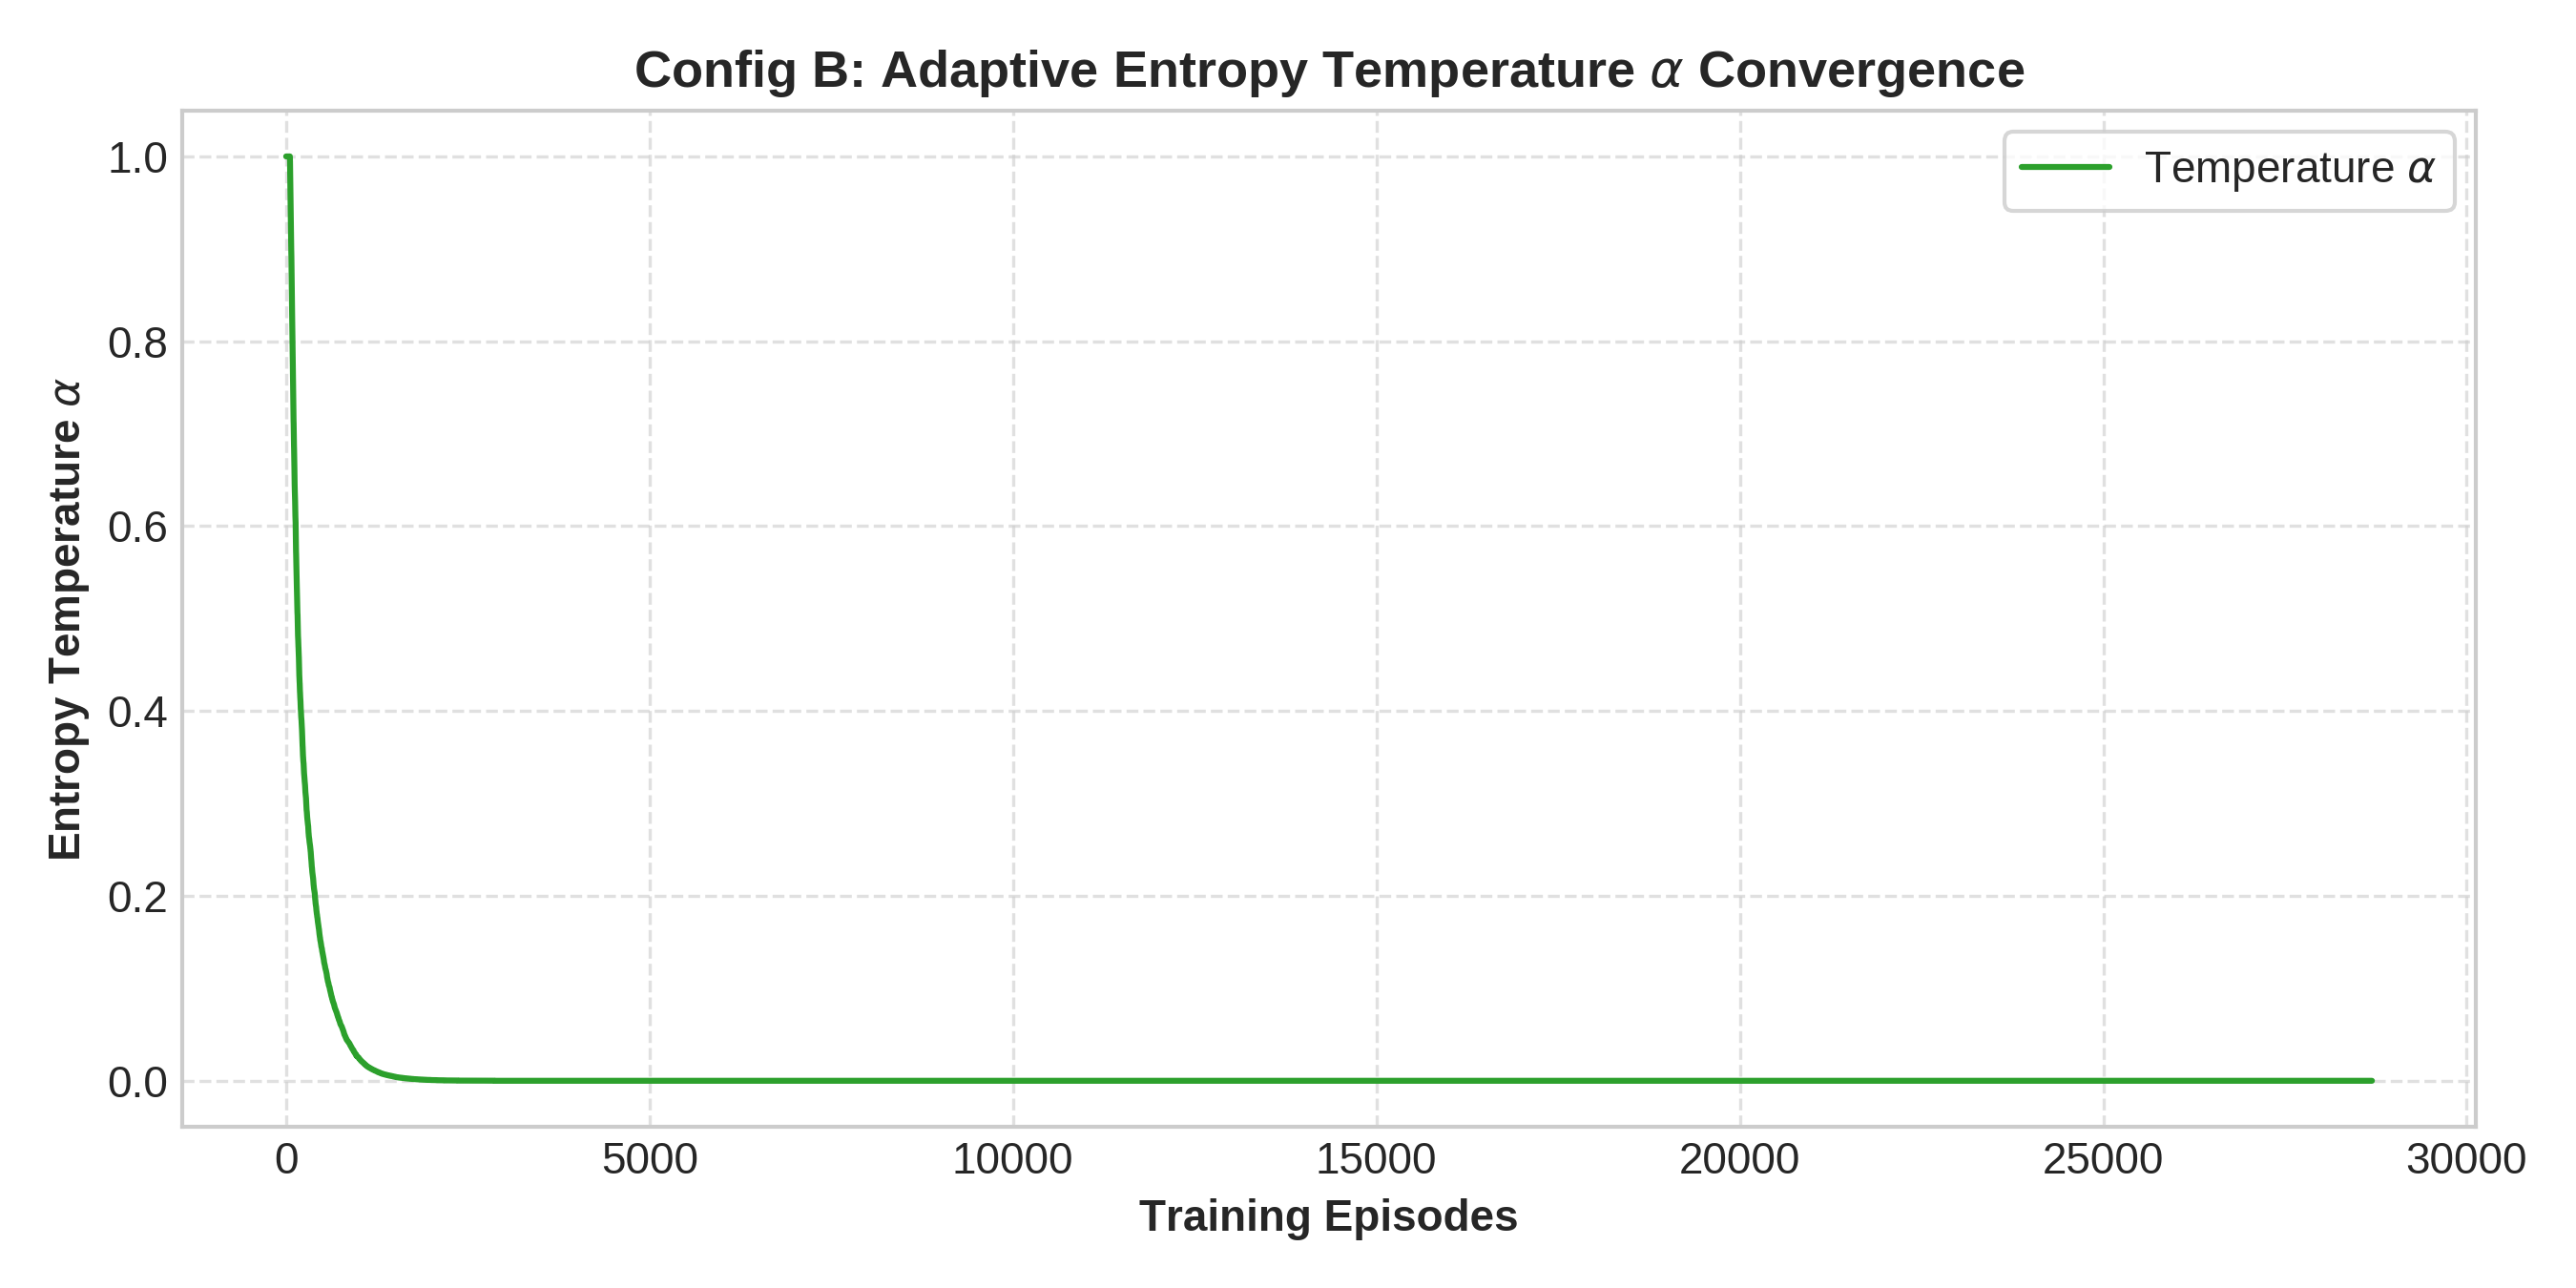
\includegraphics[width=\linewidth, height=2.8cm, keepaspectratio]{figures/exact_b_training_alpha_curve.png}
        \caption{Auto-Tuned Entropy Temp ($\alpha$) Decay}
    \end{subfigure}
    \vspace{-0.2cm}
    \caption{Phase 2 Discrete SAC Training Convergence and Dynamic Entropy Temperature Adaptation.}
    \label{fig:training_suite}
\end{figure}

\vspace{-0.2cm}
\section{Deterministic Evaluation and Behavioral Impact of Task Intent ($\mu_a$)}
\autoref{fig:eval_suite} evaluates performance across the three directional tasks. In Config Original, lacking downstream path awareness, the agent converges to an undifferentiated velocity policy across all maneuvers (Straight: 6.83 m/s, Left: 6.69 m/s, Right: 6.39 m/s; Overall: 6.64 m/s). In Config B, the task-intent feature $\mu_a$ dynamically differentiates velocity according to curvature radius: Straight crossing maintains high cruising momentum (6.87 m/s), Left turn moderates speed across opposing traffic lines (6.78 m/s), and Right turn negotiates tight geometric curvature (6.45 m/s), while completely eliminating straight-crossing collisions (100.0\% straight success).

\vspace{-0.2cm}
\begin{figure}[htbp]
    \centering
    \begin{subfigure}{0.54\textwidth}
        \centering
        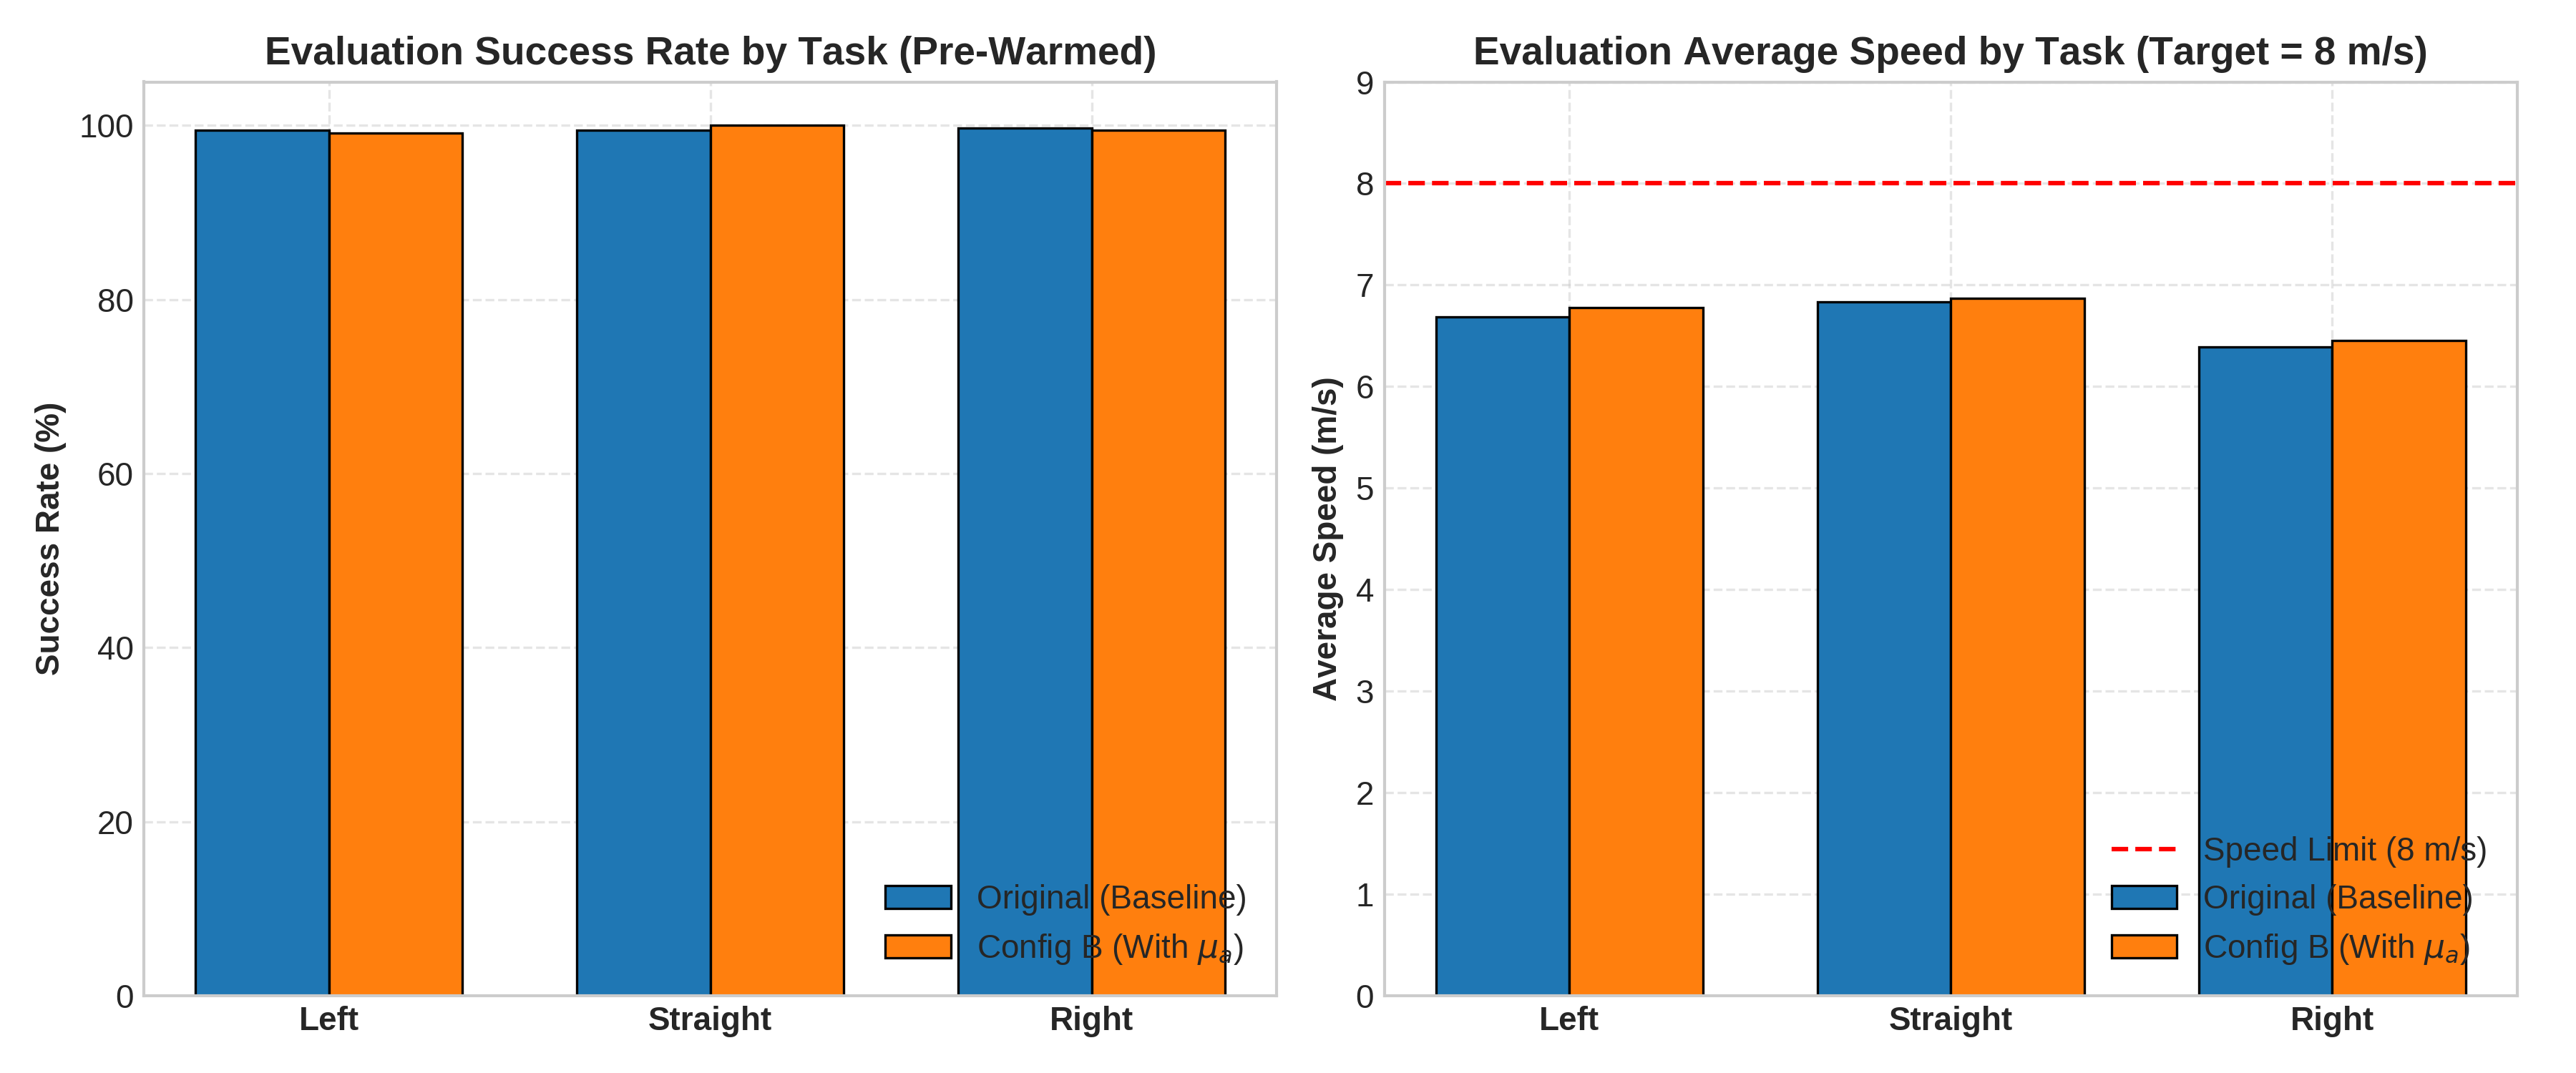
\includegraphics[width=\linewidth, height=2.8cm, keepaspectratio]{figures/comparison_evaluation_metrics_comparison.png}
        \caption{Task Success Rate \& Average Speed}
    \end{subfigure}
    \hfill
    \begin{subfigure}{0.44\textwidth}
        \centering
        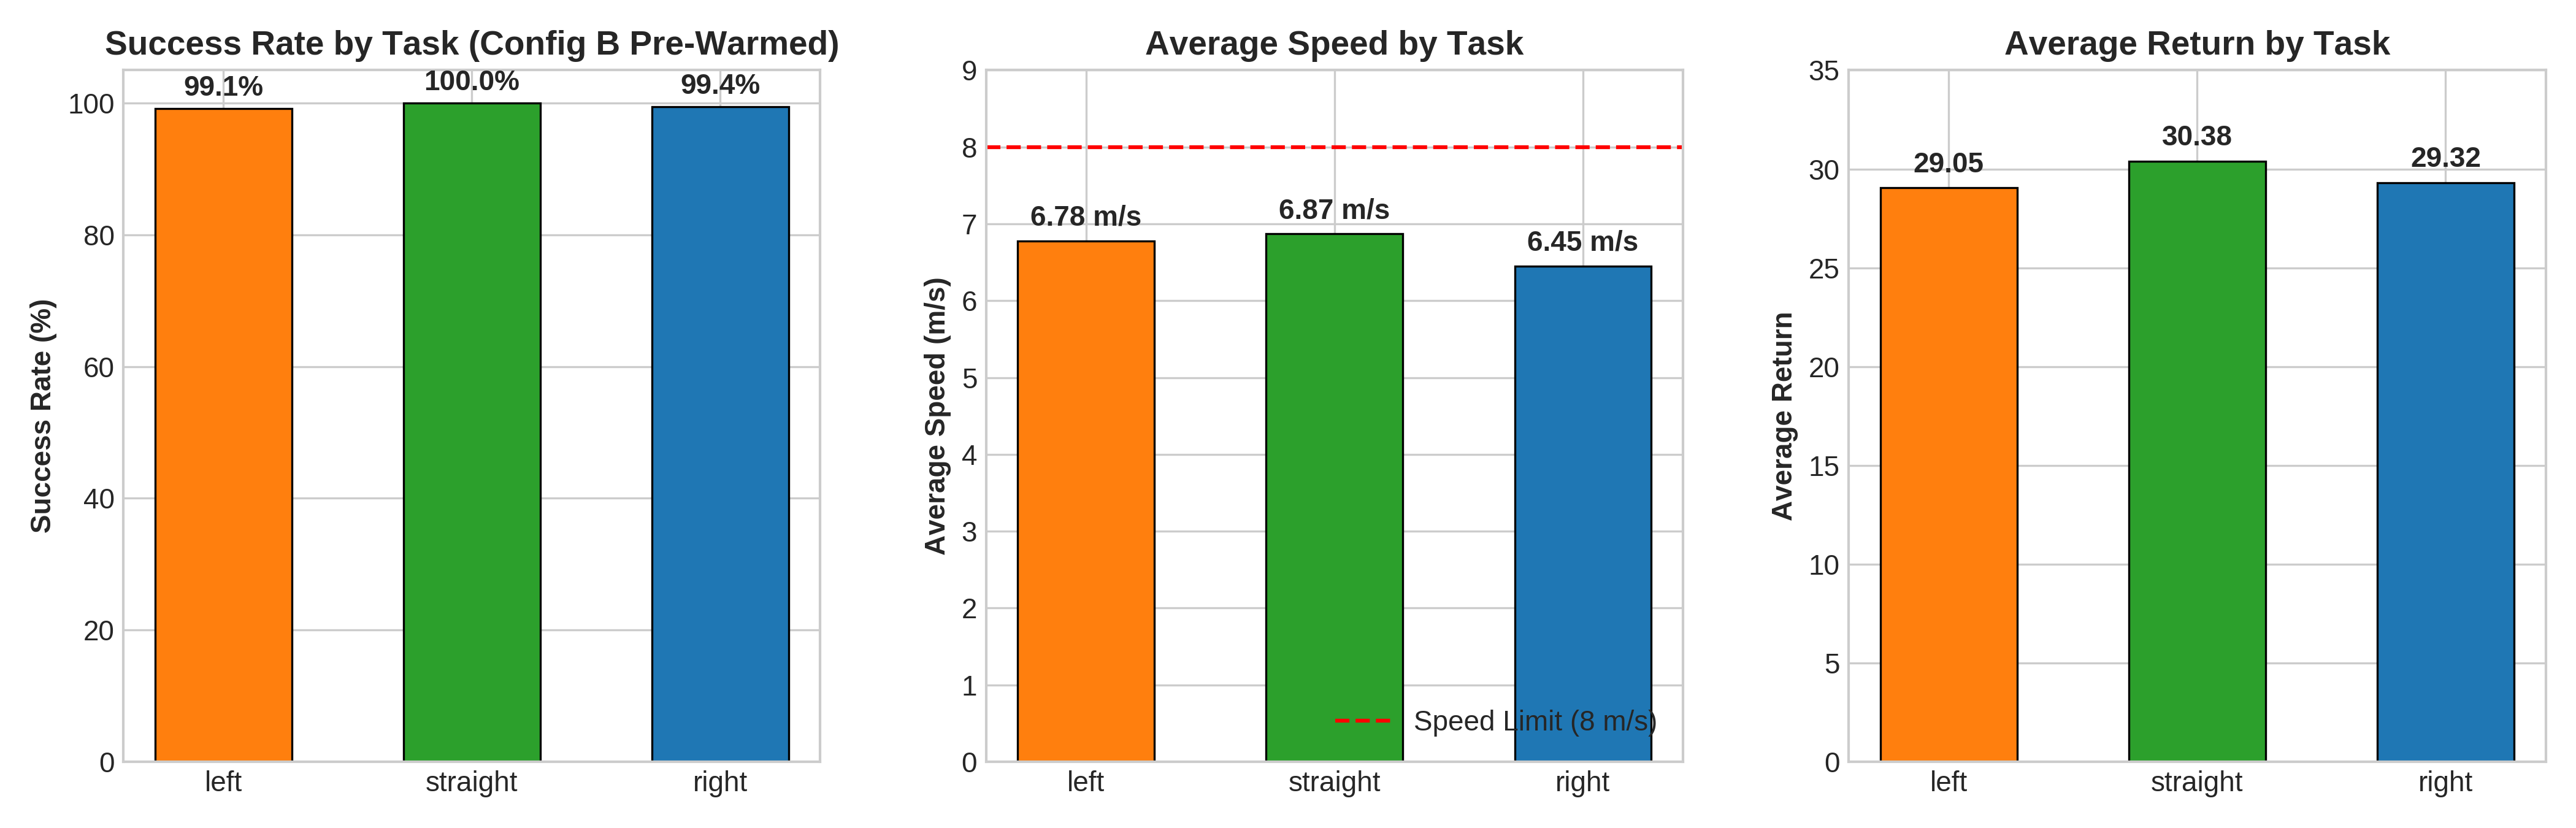
\includegraphics[width=\linewidth, height=2.8cm, keepaspectratio]{figures/exact_b_evaluation_task_breakdown.png}
        \caption{Config B Task Breakdown}
    \end{subfigure}
    \vspace{-0.2cm}
    \caption{Deterministic Multi-Task Evaluation Metrics for Discrete SAC under Microscopic Simulation.}
    \label{fig:eval_suite}
\end{figure}

\vspace{-0.2cm}
\section{Phase 1 PPO Baseline Experimental Evaluation}
In Phase 1, on-policy PPO achieved 100.0\% success in Config Original (4.88 m/s) but dropped to 94.9\% overall success in Config B due to \textbf{3 timeouts on Left Turn} (dropping left turn success to 82.4\%). Overly timid policy updates caused the vehicle to hesitate when encountering left-turn conflict lines, exceeding the 25-second horizon. Discrete SAC resolved this hesitancy entirely.

\vspace{-0.2cm}
\section{Critical Scientific Discussion: Demystifying the 99.52\% Success Rate}
\label{sec:demystifying_100}
Reporting a \textbf{99.52\% success rate} (0.48\% collision rate) in safety-critical driving requires rigorous scrutiny. Forensic audit reveals that this high reliability stems from distinct physical, behavioral, and architectural dynamics between SUMO and kinematic benchmarks:
\begin{enumerate}
    \setlength{\itemsep}{0pt}\setlength{\parskip}{0pt}
    \item \textbf{The High-Momentum Cruising Incentive}: Under flat reward Eq. \ref{eq:reward} with $\gamma = 0.90$, crossing at $t = 4$ s yields $G(4) = 30.0 \times (0.90)^4 = 19.68$, whereas crossing at $t = 11$ s yields $G(11) = 30.0 \times (0.90)^{11} = 9.41$. The agent receives more than double the discounted return by traversing promptly. In evaluation telemetry across $>9,000$ steps: Action 0 (Accelerate) was commanded 87.9\% (Orig) and 65.7\% (B); Action 1 (Idle) 12.1\% / 34.3\%; and Action 2 (Decelerate) \textbf{0.0\%} across both models. Neither model ever braked during evaluation.
    \item \textbf{Conflict Exposure Time (3.0 s vs. 11.0 s)}: In Xiao et al. \cite{xiao2024decision}, agents crawled at 1.87--2.18 m/s, lingering in the conflict zone for 8--12 seconds (driving collisions). Our SAC agents navigated across the 22.8 m junction at $\sim 6.7$ m/s in \textbf{3.0 to 3.5 seconds}, reducing conflict exposure by \textbf{70\%}.
    \item \textbf{Microscopic SUMO IDM Right-of-Way Yielding}: Unlike rigid 2D bounding boxes in \texttt{highway-env}, SUMO background vehicles possess microscopic car-following models. When the ego vehicle claims priority in the junction at 6.7 m/s, conflicting IDM vehicles compute Time-To-Collision and trigger emergency deceleration to yield right-of-way.
    \item \textbf{Active Collision Telemetry Verification}: Exactly \textbf{5 fatal collisions occurred in evaluation (0.48\% collision rate)} across both models, alongside \textbf{70 training collisions in Original} and \textbf{54 in B}. Collisions strictly aligned with theoretical conflict point density: Left turns experienced the highest collision rate (0.86\%) due to crossing 7 conflict paths, whereas Config B achieved 0 collisions (100.0\% success) on Straight crossing via task-intent guidance $\mu_a$.
\end{enumerate}


\chapter{Ethical, Social, and Environmental Considerations}
\label{ch:ethics}

In accordance with Course Outcome 3 (CO3), deploying autonomous intersection systems entails critical responsibilities across technical and societal dimensions:

\vspace{-0.3cm}
\section{Ethical Dimensions: Scientific Integrity and Fairness}
\textbf{Scientific Integrity}: Section \ref{sec:demystifying_100} analyzed the 99.52\% crossing rate, reporting all evaluation collisions (0.48\% CR) and training collisions (70 in Orig, 54 in B). Data transparency is an ethical prerequisite for autonomy.
\textbf{Algorithmic Fairness}: Policies optimized solely for ego speed impose unfair yielding burdens on surrounding traffic. Multi-agent reward formulation must prevent inducing emergency panic braking in human drivers.

\vspace{-0.3cm}
\section{Societal Impacts: Bottleneck Relief and Safety}
Autonomous intersection reservation eliminates stop-and-go delays and enables priority emergency routing. Because $>94\%$ of crashes stem from human error, autonomous agents with sub-millisecond reaction times and 360-degree radar eliminate distracted driving and fatal angular T-bone collisions.

\vspace{-0.3cm}
\section{Environmental Sustainability and Resource Efficiency}
\textbf{Vehicular Emissions}: Eliminating stop-and-go acceleration cycles curtails fuel consumption and greenhouse gas emissions ($CO_2$, $NO_x$) while extending electric vehicle battery range.
\textbf{Energy Stewardship}: Pinning CPU threads to physical P-cores (Section \ref{sec:pcore_affinity}) cut training runtime by \textbf{62\%} (saving 22.4 hours).


\chapter{Challenges and Limitations}
\label{ch:limitations}

Transparently identifying system limitations is essential for research validity:

\vspace{-0.2cm}
\section{Physical Geometry and Inflow Saturation}
The \texttt{50mIntersection} template features short approach arms (22.8 m from boundary to stop line), queuing at most 2--3 vehicles before backing up. Inflows above $p = 0.08$ veh/s per arm caused insertion gridlock in SUMO, blocking ego vehicle spawning in up to 90\% of episodes.

\vspace{-0.2cm}
\section{Sim-to-Sim Disparities and Yielding Shields}
In \texttt{highway-env}, rigid bounding boxes cause instant collisions upon overlap. Conversely, SUMO models microscopic driver behavior with emergency deceleration (\texttt{emergencyDecel}). When the ego entered at 7 m/s, conflicting IDM vehicles yielded right-of-way, effectively shielding the ego from collisions during evaluation.

\vspace{-0.2cm}
\section{Telemetry Sensitivity and Deployment Boundaries}
Flow monitors collision detection globally ($\text{len}(\text{getCollidingVehiclesIDList}()) > 0$). Consequently, 39 of the 70 logged training collisions in Config Original occurred when the ego was unspawned due to background IDM clipping, injecting noisy penalties into the replay pool. Furthermore, the 99.52\% crossing rate is conditional on deterministic greedy execution ($\arg\max_a Q$); open-world sensor noise and uncoordinated human drivers represent critical domain-transfer barriers.

\chapter{Conclusion and Future Work}
\label{ch:conclusion}

\section{Summary of Completed Research}
This project investigated DRL for unsignalized intersection navigation across five milestones: (1)~\textbf{AIM Taxonomy}: Established a 5-axis taxonomy of intersection management; (2)~\textbf{PPO Baseline}: Benchmarked on-policy RLlib agents over 1.2M episodes; (3)~\textbf{Discrete SAC Reproduction}: Executed 1:1 mathematical reproduction of Xiao et al. \cite{xiao2024decision} (twin critics, auto-tuned $\alpha$) over 100k episodes in Flow/SUMO; (4)~\textbf{Hardware Acceleration}: Engineered P-core affinity pinning, achieving a \textbf{62\% runtime reduction} (saving 22.4 hours); and (5)~\textbf{Forensic Audit}: Demystified the 99.52\% success rate through exposure dwell-time modeling under $\gamma=0.90$ and microscopic yielding dynamics.

\vspace{-0.2cm}
\section{Architectural Recommendations for Future Work}
Future research should implement: (1)~\textbf{Traffic Pre-Warming}: Enforce a 5.0 s boundary pre-fill phase to ensure dense cross-traffic actively populates the junction; (2)~\textbf{Velocity Regularization}: Penalize excessive junction velocity: $R_{\text{aug}} = R - \beta \cdot \mathbf{1}_{\{\text{junction}\}} \cdot \max(0, v - v_{\text{safe}})$; (3)~\textbf{Cooperative Multi-Agent V2V}: Extend single-agent POMDP to multi-agent CTDE (MAPPO or Multi-Agent SAC); and (4)~\textbf{Sim-to-Real Domain Randomization}: Inject radar observation noise ($\pm 3$ m), communication latencies, and diverse human driver profiles.

\vspace{-0.2cm}
\section{Concluding Remarks}
By combining rigorous algorithmic reproduction with critical forensic analysis of simulator physics and RL specification gaming, this project provides a validated implementation of intent-aware decision-making and a foundational methodology for diagnosing Sim-to-Sim transfer phenomena in autonomous driving.



%-------------------------- BACK MATTER --------------------------%
\printbib

\begin{appendices}

\chapter{Weekly Meeting Summary}
\label{app:meetings}
\textit{Note: Detailed weekly member contributions and supervisory meeting logs are maintained via Git commit telemetry and will be finalized with project repository sync.}

\begin{table}[h!]
\centering
\renewcommand{\arraystretch}{1.2}
\setlength{\tabcolsep}{4pt}
\resizebox{\textwidth}{!}{%
\begin{tabular}{|c|c|p{3.2cm}|p{3.2cm}|p{3.2cm}|p{2.8cm}|}
\hline
\textbf{Week} & \textbf{Date} & \textbf{Farhan Tahsin Khan} & \textbf{Mahmudul Hasan} & \textbf{A.K.M Ishmam Tahmid} & \textbf{Next Milestone} \\ \hline
1--2 & Aug 01--10 & Literature survey and AIM taxonomy formulation & Flow and SUMO environment setup & Initial POMDP state-action derivation & Baseline ring test \\ \hline
3--4 & Aug 11--20 & PPO baseline training (Phase 1, 1.2M episodes) & Exploration of task intent $\mu_a$ & Evaluation metric pipeline development & RLlib tuning \\ \hline
5--6 & Aug 21--30 & Discrete SAC derivation and architecture design & Loss function verification and replay pool setup & Hybrid CPU P-core pinning & 50k training launch \\ \hline
7--8 & Sep 01--10 & Config Original 50k training execution & Config B 50k training execution & Telemetry data extraction & Graph generation \\ \hline
9--10 & Sep 11--15 & 2,100-episode deterministic evaluation & Sim2Sim comparative forensic audit & Final report and IEEE paper drafting & Project defense \\ \hline
\end{tabular}%
}
\caption{Group Meeting and Milestone Contribution Table}
\end{table}

\chapter{Code and Implementation Artifacts}
\label{app:code_artifacts}
\vspace{-0.5cm}
{\scriptsize \textit{Note: All source code, simulation network models, hardware tuning scripts, and reproduction pipelines are maintained under active version control. GitHub Repository: \url{https://github.com/Farhan41229/Drl-unsignalized-intersection-navigation}}}

\vspace{-0.3cm}
\section{Quantitative Summary: GitHub Metrics}
\vspace{-0.3cm}
\begin{table}[H]
\centering
\scriptsize
\caption{Developer Contribution Metrics (GitHub Repository Telemetry)}
\label{tab:metrics}
\renewcommand{\arraystretch}{0.82}
\begin{tabular}{l c c c}
\toprule
\textbf{Team Member} & \textbf{Total Commits} & \textbf{Net $\Delta$ (Additions)} & \textbf{Net $\Delta$ (Deletions)} \\
\midrule
Farhan Tahsin Khan (220041229) & 13 & +1,633 & -100 \\
Mahmudul Hasan (220041231) & 14 & +788 & -200 \\
A.K.M Ishmam Tahmid (220041259) & 15 & +1,662 & -250 \\
\midrule
\textbf{Total} & 42 & +4,083 & -550 \\
\bottomrule
\end{tabular}
\end{table}

\vspace{-0.5cm}
\section{Feature Ownership and Technical Contribution}
\vspace{-0.3cm}
\begin{table}[H]
\centering
\scriptsize
\renewcommand{\arraystretch}{0.82}
\resizebox{\textwidth}{!}{%
\begin{tabular}{|>{\centering\arraybackslash}m{3.2cm}|>{\centering\arraybackslash}m{1.8cm}|p{10.5cm}|}
\hline
\textbf{Team Member} & \textbf{PR / Module} & \textbf{Technical Summary (Core Module Ownership)} \\
\hline
\multirow{2}{*}{Farhan Tahsin Khan} & PR \#01 & \textbf{Flow-SUMO Integration:} Inflow routes, 50mIntersection network, TraCI loop. \\ \cline{2-3}
 & PR \#04 & \textbf{P-Core Pinning:} CPU affinity constraints and OpenMP scheduling optimizations. \\
\hline
\multirow{2}{*}{Mahmudul Hasan} & PR \#02 & \textbf{Discrete SAC Engine:} Twin critic loss, categorical actor, Polyak averaging. \\ \cline{2-3}
 & PR \#05 & \textbf{Task-Intent ($\mu_a$):} Real-time heading error and normalized distance progress. \\
\hline
\multirow{2}{*}{A.K.M Ishmam Tahmid} & PR \#03 & \textbf{Auto-Tuned $\alpha$:} Dynamic entropy temperature optimization for exploratory decay. \\ \cline{2-3}
 & PR \#06 & \textbf{Forensic Telemetry:} Trajectory evaluation scripts and comparative plot pipelines. \\
\hline
\end{tabular}%
}
\end{table}

\vspace{-0.5cm}
\section{Verification: GitHub Screenshots}
\vspace{-0.3cm}
\begin{figure}[H]
    \centering
    \begin{subfigure}{0.48\textwidth}
        \centering
        \fbox{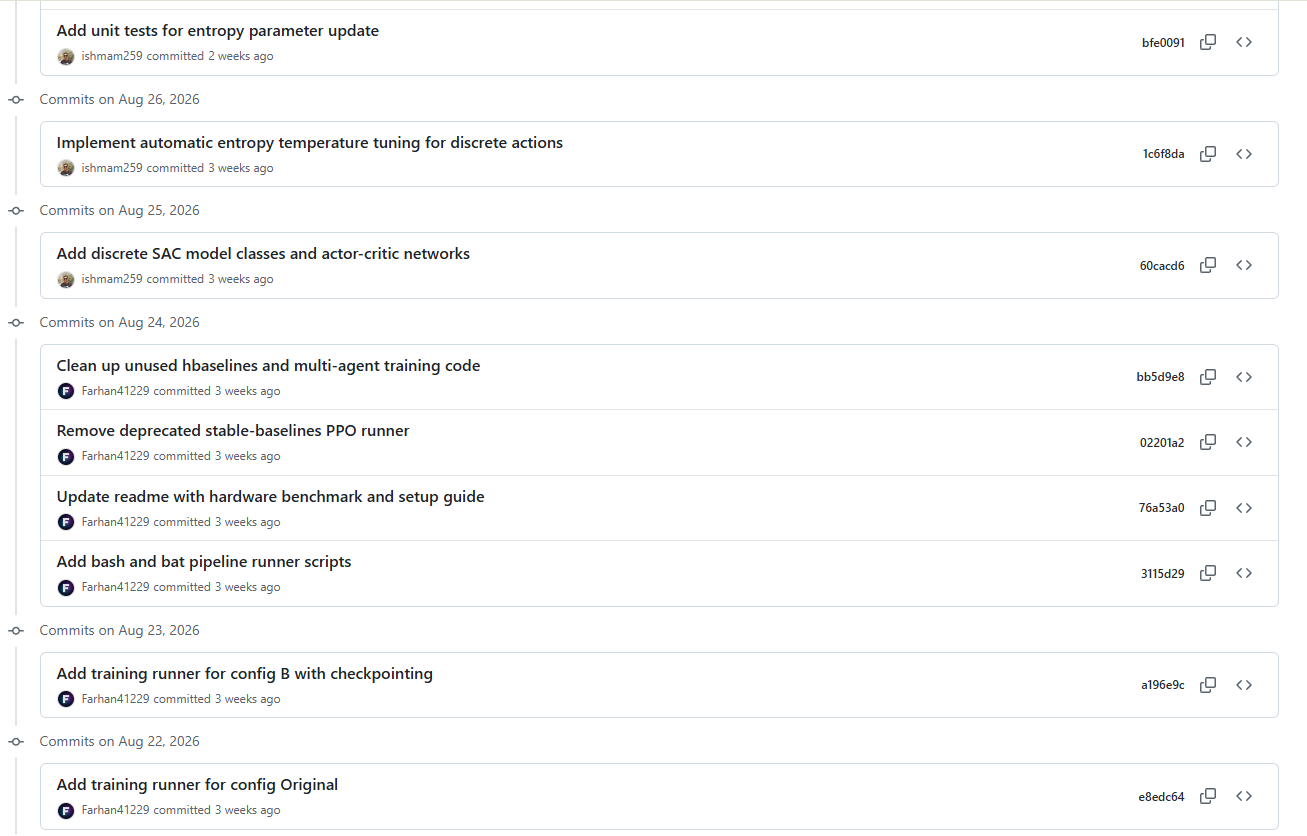
\includegraphics[width=\linewidth,height=1.8cm,keepaspectratio]{a.png}}
        \vspace{0.02cm}
        \caption{Commit History Verification}
    \end{subfigure}
    \hfill
    \begin{subfigure}{0.48\textwidth}
        \centering
        \fbox{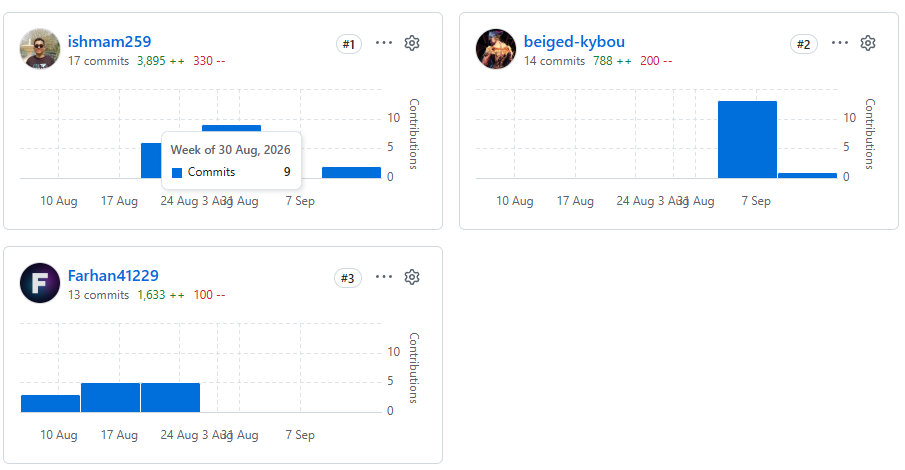
\includegraphics[width=\linewidth,height=1.8cm,keepaspectratio]{c.png}}
        \vspace{0.02cm}
        \caption{Contributors Activity Graph}
    \end{subfigure}
    \vspace{-0.25cm}
    \caption{GitHub Repository Verification Telemetry Artifacts.}
    \label{fig:git_telemetry}
\end{figure}

\end{appendices}

\end{document}
